% =========
% CHƯƠNG 8
% =========
\OpenGrid

\ParallelChapter
  {Reasoning with Statistics and Probability}
  {Luận với thống kê và xác suất}
  {}

\TriPara
  {
    \EN{In our increasingly data-intensive world, statistics is one of the most important areas of the mathematical sciences for helping students make sense of the information all around them, as well as for preparing them for further study in a variety of disciplines (e.g., the health sciences, the social sciences, and environmental science) for which statistics is a fundamental tool for advancing knowledge. Competence in the Standards found in \emph{Principles and Standards} (NCTM 2000a) depends on a thorough and deep understanding of the foundations of statistics and probability, and of the connections between statistics and probability. Taken together, \emph{Principles and Standards} and the American Statistical Association's report \emph{Guidelines for Assessment and Instruction in Statistics Education} (GAISE) (Franklin et al. 2007) describe statistical problem solving as an investigative process that involves the following four components:

    \begin{itemize}
      \item Formulating a question (or questions) that can be addressed with data
      
      \item Designing and employing a plan for collecting data
      
      \item Analyzing and summarizing the data
      
      \item Interpreting the results from the analysis, and answering the question on the basis of the data
    \end{itemize}}
  }
  {
    \VI{Trong thế giới ngày càng dựa nhiều vào dữ liệu như hiện nay, thống kê là một trong những lĩnh vực quan trọng nhất của các khoa học toán học trong việc giúp học sinh hiểu thông tin xung quanh mình, đồng thời chuẩn bị cho các em tiếp tục học tập trong nhiều ngành khác nhau (chẳng hạn khoa học sức khỏe, khoa học xã hội, và khoa học môi trường), những ngành mà thống kê là công cụ nền tảng để phát triển tri thức. Việc đạt được năng lực theo các Chuẩn được nêu trong \emph{Principles and Standards} (NCTM 2000a) phụ thuộc vào sự hiểu biết vững chắc và sâu sắc về nền tảng của thống kê và xác suất, cũng như về mối liên hệ giữa thống kê và xác suất. Kết hợp lại, \emph{Principles and Standards} và báo cáo của Hiệp hội Thống kê Hoa Kì mang tên \emph{Guidelines for Assessment and Instruction in Statistics Education} (GAISE) (Franklin et al. 2007) mô tả việc giải quyết vấn đề thống kê như quá trình điều tra gồm bốn thành phần sau:

    \begin{itemize}
      \item Hình thành câu hỏi, hoặc nhóm câu hỏi, có thể xử lí bằng dữ liệu

      \item Thiết kế và triển khai kế hoạch thu thập dữ liệu

      \item Phân tích và tóm tắt dữ liệu
      
      \item Diễn giải kết quả phân tích, và trả lời câu hỏi trên cơ sở dữ liệu
    \end{itemize}}
  }{\NOTE{}}

\TriPara
  {
    \EN{The common thread throughout the statistical problem-solving process is the focus on making sense of, and reasoning about, variation in data. The goal is not only to solve problems in the presence of variation but also to provide a measure of how much the variation might affect the solution. This process provides a framework for teaching and learning statistics in school, and meaningful tasks that employ this process should permeate the statistical education of our students.}
  }
  {
    \VI{Mạch xuyên suốt toàn bộ quá trình giải quyết vấn đề thống kê là sự tập trung vào việc hiểu và luận về sự biến thiên trong dữ liệu. Mục tiêu không chỉ là giải quyết các bài toán khi có biến thiên, mà còn là đưa ra một thước đo cho biết biến thiên ấy có thể ảnh hưởng đến lời giải ở mức nào. Quá trình này cung cấp một khuôn khổ cho việc dạy và học thống kê trong nhà trường, và những nhiệm vụ có ý nghĩa vận dụng quá trình ấy cần hiện diện xuyên suốt trong giáo dục thống kê ở học sinh.}
  }
  {
    \NOTE{``Sự biến thiên'' là trọng tâm cốt lõi của luận thống kê. Thống kê không tìm cách loại bỏ biến thiên, mà học cách hiểu, mô tả và luận về biến thiên như đặc trưng tất yếu của dữ liệu trong thế giới thực.

    Việc nhấn mạnh rằng mục tiêu không chỉ là tìm lời giải, mà còn là đánh giá mức độ ảnh hưởng của biến thiên đối với lời giải, cho thấy điểm đặc trưng của tư duy thống kê: kết quả không chỉ được xem xét ở bản thân giá trị thu được, mà còn ở mức độ giá trị ấy có thể bị tác động bởi sự biến thiên trong dữ liệu.

    Quá trình giải quyết vấn đề thống kê không chỉ là mô hình kĩ thuật, mà còn là khuôn khổ sư phạm cho việc dạy và học thống kê. Theo đó, các nhiệm vụ học tập có ý nghĩa cần thường xuyên đặt học sinh trước dữ liệu có biến thiên, để các em phải hiểu và luận về biến thiên ấy, thay vì chỉ thực hiện các thao tác tính toán rời rạc.}
  }

\TriPara
  {
    \EN{Key elements of reasoning and sense making with statistics and probability include the following:
    \begin{itemize}
      \item \emph{Data analysis.} Gaining insight about a solution to a statistics question by collecting data and describing features of the data through the use of graphical and tabular representations and numerical summaries. (The interpretation of results in data analysis encompasses both empirical and informal levels of reasoning, as described in the progression of reasoning in chapter 2.)
      
      \item \emph{Modeling variability.} Developing probability models to describe the long-run behavior of observations of a random variable.
      
      \item \emph{Connecting statistics and probability.} Recognizing probability as an essential tool of statistics; understanding the role of probability in statistical reasoning.
      
      \item \emph{Interpreting designed statistical studies.} Drawing appropriate conclusions from data in ways that acknowledge random variation. (Interpreting results from designed statistical studies involves statistical inference and other more formal levels of statistical reasoning.)
    \end{itemize}
    We address these key elements in more detail in the following sections.}
  }
  {
    \VI{Các yếu tố then chốt của luận và hiểu trong thống kê và xác suất gồm có: \vspace{\baselineskip}
    \begin{itemize}
      \item \emph{Phân tích dữ liệu.} Hình thành hiểu biết về lời giải cho câu hỏi thống kê bằng cách thu thập dữ liệu và mô tả đặc trưng của dữ liệu thông qua biểu diễn bằng đồ thị, biểu diễn bằng bảng và tóm tắt số. (Việc diễn giải kết quả trong phân tích dữ liệu bao hàm cả mức độ luận thực nghiệm và phi hình thức, như đã được mô tả trong Tiến trình phát triển của luận ở Chương 2.)
      
      \item \emph{Mô hình hóa biến thiên.} Phát triển mô hình xác suất để mô tả hành vi dài hạn của các quan sát từ biến ngẫu nhiên.
      
      \item \emph{Kết nối thống kê và xác suất.} Nhận ra xác suất là công cụ thiết yếu của thống kê; hiểu biết vai trò của xác suất trong luận thống kê. \vspace{\baselineskip}
      
      \item \emph{Diễn giải các nghiên cứu thống kê có thiết kế.} Rút ra kết luận thích hợp từ dữ liệu theo cách có tính đến biến thiên ngẫu nhiên. (Việc diễn giải kết quả từ nghiên cứu thống kê có thiết kế bao hàm suy luận thống kê và các mức độ luận thống kê hình thức hơn.)
    \end{itemize}
    Chúng tôi sẽ trình bày chi tiết hơn các yếu tố then chốt này trong các phần tiếp theo.}
  }{\NOTE{}}

\ParallelSection
  {Data Analysis}
  {Phân tích dữ liệu}
  {}

\TriPara
  {
    \EN{Data analysis is more than simply the analysis of data. Data analysis includes all four components described in the process of statistical problem solving. Data are observations or measurements collected on one or more variables to address a statistical question. In statistics, a variable is any characteristic for which individual observations can be expected to take different values. Consequently, data vary and, once collected, need to be summarized in ways that foster meaningful insights for addressing the question under study. The analysis of data includes exploring various representations of the \emph{data distribution} to summarize and describe patterns and relationships in the variation and to identify deviations from a pattern. Technology provides the opportunity to examine various representations of the data distribution and to identify important features of the distribution. In data analysis, the interpretation of results includes both empirical and informal levels of reasoning. Because both numerical data and numerical summaries of data are used in data analysis, statistics has connections with the Numbers and Measurements strand described in chapter 4, particularly the key elements of \emph{reasonableness of answers and measurements and approximations and error}.}
  }
  {
    \VI{Phân tích dữ liệu không chỉ đơn thuần là thao tác phân tích dữ liệu theo nghĩa hẹp. Phân tích dữ liệu bao gồm đầy đủ bốn thành phần được mô tả trong quá trình giải quyết vấn đề thống kê. Dữ liệu là quan sát hoặc phép đo được thu thập đối với một hoặc nhiều biến nhằm xử lí câu hỏi thống kê. Trong thống kê, biến là bất kì đặc trưng nào mà từng quan sát có thể nhận giá trị khác nhau. Vì thế, dữ liệu có biến thiên; và sau khi được thu thập, dữ liệu cần được tóm tắt theo cách giúp hình thành hiểu biết có ý nghĩa cho việc xử lí câu hỏi đang xét. Phân tích dữ liệu bao gồm việc khảo sát nhiều biểu diễn khác nhau của \emph{phân bố dữ liệu} nhằm tóm tắt và mô tả mẫu hình và quan hệ trong sự biến thiên, cũng như nhận diện những lệch khỏi mẫu hình. Công nghệ tạo cơ hội xem xét nhiều biểu diễn khác nhau của phân bố dữ liệu và nhận diện đặc trưng quan trọng của phân bố. Trong phân tích dữ liệu, việc diễn giải kết quả bao gồm cả mức độ luận thực nghiệm và phi hình thức. Vì cả dữ liệu số lẫn tóm tắt số của dữ liệu đều được sử dụng trong phân tích dữ liệu, thống kê có liên hệ với mạch Số và đo lường được trình bày ở Chương 4, đặc biệt là các yếu tố then chốt \emph{tính hợp lí của đáp số và phép đo}, cùng với \emph{xấp xỉ và sai số}.}
  }{\NOTE{}}

\TriPara
  {
    \EN{Example 19 shows how statistical procedures for analyzing data that are developed in earlier grades continue to be useful tools for making sense of, and reasoning about, data in high school. Example 19 illustrates organizing and interpreting a solution and recognizing the scope of inference for a statistical solution. A detailed description of this activity is given in Kader and Mamer (2008).}
  }
  {
    \VI{Ví dụ 19 cho thấy các thủ tục thống kê dùng để phân tích dữ liệu, vốn được phát triển ở các lớp trước, tiếp tục là công cụ hữu ích để hiểu và luận về dữ liệu ở trung học phổ thông. Ví dụ 19 minh họa việc tổ chức và diễn giải một lời giải, đồng thời nhận ra phạm vi suy luận của lời giải thống kê. Mô tả chi tiết về hoạt động này được trình bày trong Kader and Mamer (2008).}
  }{\NOTE{}}

\TriExample
  {
    Meaningful Words (A)
  }
  {
    \begin{center}
      Adapted from WGBH Educational\\ Foundation (2001)
    \end{center}\vspace{.2\baselineskip}

    \textbf{Task}

    Scientists are interested in human recall and memory. Is it easier to memorize words that have ``meaning?'' To study this problem, two lists of $20$ three-letter ``words'' were used. One list contained meaningful words (e.g., CAT, DOG), whereas the other list contained nonsense words (e.g., ATC, ODG). A ninth-grade class of thirty students was randomly divided into two groups of fifteen students. One group was asked to memorize the list of meaningful words; the other group was asked to memorize the list of nonsense words. The number of words correctly recalled by each student was tabulated, and the resulting data are as follows:

    Number of meaningful words recalled: $12$, $15$, $12$, $12$, $10$, $3$, $7$, $11$, $9$, $14$, $9$, $10$, $9$, $5$, $13$ 

    Number of nonsense words recalled: $4$, $6$, $6$, $5$, $7$, $5$, $4$, $7$, $9$, $10$, $4$, $8$, $7$, $3$, $2$

    \begin{enumerate}
      \item Provide a display for summarizing and comparing these data sets.
      
      \item On the basis of your display, what observations can be made regarding how the students assigned the meaningful words performed compared with how the students assigned the nonsense words performed? Write a paragraph summarizing what the data and your analysis reveal about the question ``Is it easier to memorize words that have meaning?''
    \end{enumerate}

    \textbf{In the Classroom (Ninth-Grade Mathematics Class)}

    Several groups of students created comparative dotplots for the data, as shown below.

    \begin{center}
      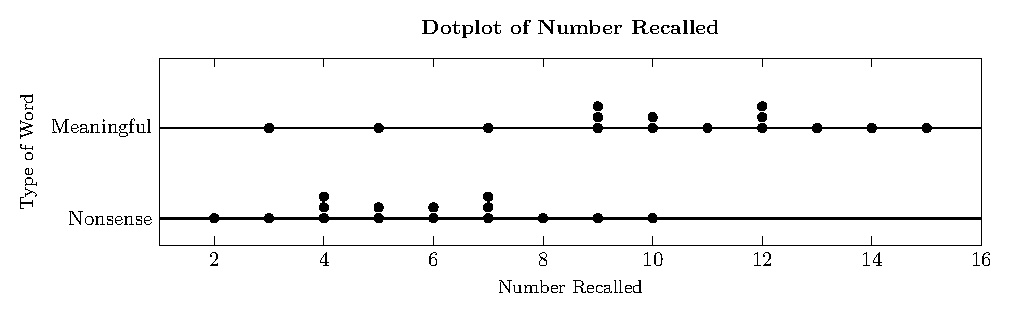
\includegraphics[width=.92\linewidth]{../figures/fhsm_2009_p75_1.pdf}
    \end{center}

    \begin{scriptlist}
      \item [Teacher:] Looking at the dotplots, for which type of words did students generally have better recall? How do you know? Give some specific reasons for your answer.
      
      \item [Student A:] A lot of students with the meaningful words did better. The highest number recalled is ten for the students with the nonsense words. Seven of the students with meaningful words recalled more than ten words, and ten is the best for all the students with the nonsense words.
  
      \item [Student B:] Yes, but some of the students with the meaningful words did not do very well, either. One recalled only three words; another, only fi ve words; and another, only seven words. These seem low for the meaningful words.
      
      \item [Student C:] Yes, and there are some gaps in the low end of the meaningful-words data distribution but not so much in the nonsense-words distribution. A lot of the students with the nonsense words recalled between three and seven words, and only a few of the students with the meaningful words recalled between three and seven words.
      
      \item [Teacher:] Can you be more specific?\vspace{\baselineskip}
      
      \item [Student C:] Well, three out of the fifteen students with the meaningful words recalled between three and seven words. That's only $20$ percent. For the students using the nonsense words, eleven out of fifteen, more than $73$ percent, recalled that many. If you add the student who only recalled two nonsense words, twelve out of these fifteen students, that's $80$ percent, recalled between two and seven words, whereas only $20$ percent of the students with the meaningful words were this low. In fact, all fifteen students using the nonsense words recalled between two and ten words, but only eight students with the meaningful words were this low. 
  
      \item [Teacher:] That's the same as what student A said, seven of the fifteen students using the meaningful-words list recalled more words than any of the students using the nonsense-words list. That means close to half the students memorizing the meaningful words did better than all students with the nonsense words.
      
      \item [Teacher:] Let's try to identify a typical value for the number of words recalled for each list. What quantity would you propose?
      
      \item [Student D:] We could find the average number recalled for each list.
      
      \item [Teacher:] Why do you propose the average, which is also called the mean?
      
      \item [Student D:] Well, it seems like we always find the mean whenever we want to know a typical value.
  
      \item [Student E:] Yes, sometimes the mean is good. But sometimes we use the median for a typical value.\vspace{\baselineskip}
      
      \item [Teacher:] In this case, does it matter which one you use?\vspace{\baselineskip}
      
      \item [Student E:] Well, in the dotplot for the meaningful words, three of the values look kind of small. I think these three values might make the mean smaller than what's typical. So I would use the median instead of the mean.
      
      \item [Teacher:] Very good. When we see a graph of data like the dotplot for the meaningful words, we say the shape of the data distribution is skewed to the left. Like student E said, when a data distribution is skewed left, the mean is often smaller than what one might think of as typical for the data. For this reason, the median might provide a better indication of how many words were typically recalled by students with the meaningful list. So, what would you propose for a typical value for the number of words recalled by students with the nonsense-words list?
      
      \item [Student E:] The data distribution for the nonsense list looks pretty even. I think this indicates it has a symmetrical shape. So you could probably use either the mean or the median for these data. Since we are using the median for the meaningful words, and it would not make sense to compare the mean of one group to the median of another group, I would use the median for the nonsense words as well.
      
      \item [Teacher:] What do the rest of you think? What happens when we use the medians?
      
      \item [Student D:] My calculator gives the median for the meaningful words as $10$, and for the nonsense words the median is $6$. 
      
      \item [Teacher:] What if we did not have the data values, but only knew the medians? What do the medians tell us about the data?
      
      \item [Student D:] The median divides the data in half.
      
      \item [Teacher:] Yes, so if the median is ten words for the data on meaningful words, what can we say about the rest of the data?
      
      \item [Student F:] About half the students assigned to the meaningful-words list remembered fewer than ten words, and about half remembered more than ten words.
      
      \item [Teacher:] Comparing the two medians, what would you conclude?
      
      \item [Student F:] The median for the meaningful words is ten words, but the median for the nonsense words is six words. Ten is higher than six, so students with meaningful words typically did better than the students with nonsense words.
      
      \item [Teacher:] This is an interesting observation. Another way of looking at this is to say that the difference between the medians is four words. So students with the meaningful words typically recalled four more words than students with the nonsense list.
      
      \item [Teacher:] If only the medians are reported for these data, what information about the number of words recalled is missing?
      
      \item [Student G:] If all you know is the median, you don't know the actual number recalled for each student. Take the data for the meaningful words. If all I know is that the median number recalled is ten words, I don't really know about the different values that actually occurred. For example, looking at the student who remembered only three words, three words is a lot different from ten words.
      
      \item [Teacher:] So, student G, what is the idea you talking about called?
      
      \item [Student G:] The number of words recalled is not the same for each student. I think this is the idea of variability in the data, which we have talked about before.
      
      \item [Teacher:] Yes, you are correct. In statistics, we are interested in representing the data with a typical value, such as the median, but we are also interested in summarizing the amount of variability in the data, as well. Does anyone have any suggestions for how we might do this?
  
      \item [Student H:] We could find the ranges. I think this tells us something about how much variability there is. The range is 12 for the meaningful list. The range for the nonsense list is $8$.\vspace{\baselineskip}
      
      \item [Teacher:] So, what do the ranges suggest about the variation in the data?
      
      \item [Student H:] The biggest difference between any two values from the meaningful list is twelve words, but the biggest difference between any two values from the nonsense list is eight words. This says that there is more variability in the number of words recalled on the meaningful words list than on the nonsense words list.
      
      \item [Student I:] Yes, but the smallest value from the meaningful words seems really small. For this reason, I don't think I would use the ranges. Instead, I think we should find the quartiles and use the interquartile ranges (IQR) instead. Then I am comparing the amount of variation for the middle portions of each group.
      
      \item [Teacher:] How do you find the IQR?
      
      \item [Student I:] First you have to find the first and third quartiles for each group of data. Then you find the range between the quartiles. You subtract the first quartile from the third quartile.
      
      \item [Teacher:] OK. Everyone find the quartiles and the interquartile ranges.
  
      \item [Student J:] For the meaningful words, my calculator gives the first quartile as nine words and the third quartile as twelve words. So the IQR is three words. For the nonsense words, the first quartile is four words and the third quartile is seven words. So the IQR is three words. The IQRs are the same, so there are similar amounts of variation in the middle $50$ percent of the data for both the meaningful words and the nonsense words.
      
      \item [Student K:] My calculator gives five quantities for each group-the minimum, the first quartile, the median, the third quartile, and the maximum. I think we can get a graph called a box-and-whiskers plot by using these five numbers.
      
      \item [Teacher:] Yes, you can. When you include an outlier analysis, it is called a modified boxplot.
    \end{scriptlist}\vspace{\baselineskip}

    The class used results from a calculator to produce the following comparative modified boxplots:

    \begin{center}
      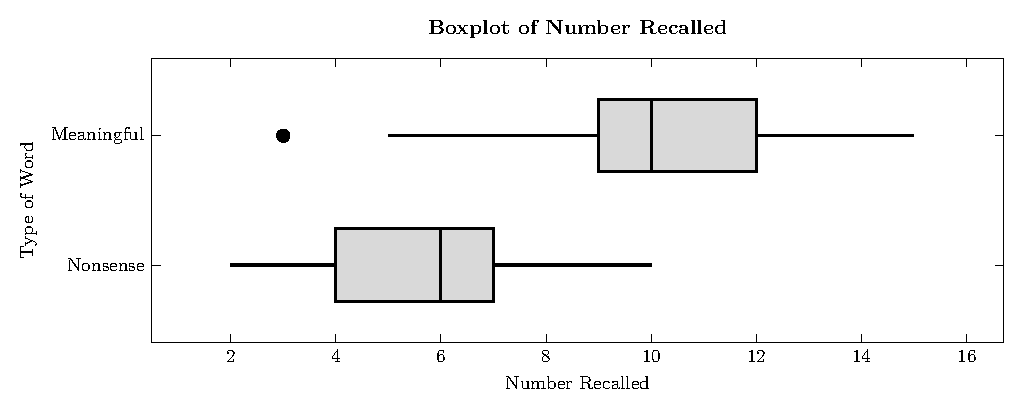
\includegraphics[width=.92\linewidth]{../figures/fhsm_2009_p79_1.pdf}
    \end{center}

    \begin{scriptlist}
      \item [Teacher:] Can you use the results from the boxplots to summarize our discussions about this question?
      
      \item [Student M:] Students with the list of meaningful words generally recalled more words. The maximum number of words recalled for the students with the nonsense list is ten. Ten is the median number recalled for the meaningful list, so about half the students with the meaningful words recalled more words than any of the student with the nonsense words. With the meaningful words, one student recalled only three words, and this score is an outlier and somewhat lower than expected when compared to the other data. The median number recalled with the meaningful words is ten, which is four more words than the median number recalled from the nonsense words. Excluding the outlier from the meaningful-words data, both groups appear to have similar amounts of variation. The IQR for each group is $3$, indicating that for both meaningful and nonsense words the number of words recalled within the middle $50$ percent differ by no more than three words.
      
      \item [Teacher:] What do these results suggest about memory and meaning?
      
      \item [Student N:] Since students with the meaningful words seemed to do better, these data suggest it is easier to memorize words that have meaning.
      
      \item [Teacher:] Do you think it would be appropriate to say that all ninth graders would get exactly the same results?
      
      \item [Student O:] Sure, it's easier to memorize words that have meaning.
      
      \item [Student P:] Well, we would not get exactly the same scores! But we might still see that words with meaning will be easier to memorize.
      
      \item [Teacher:] We have to be careful about our scope of inference, or trying to generalize these results to other ninth graders based on these data. The scope of inference depends on whether or not the studied class is representative of all ninth-grade classes. As we don't know how the class was selected, we should not try to generalize the results to all ninth-grade classes or to all ninth graders. If a group of ninth-grade students is selected at random, then we might try to generalize these results to all ninth graders.
      
      \item [Student Q:] But I thought they used randomness in the study.
      
      \item [Teacher:] Yes, they did. However, randomness was used in assigning the students to the different groups. The reason for using random assignment is to produce two comparable groups. For example, you would not want all students who are good at memorizing in one group. By randomly assigning the students to the two groups, we hope to balance the effects from not only students' memorizing ability but from any other variables that might be related to the number of words recalled. Although random assignment does not guarantee similar groups, there is a high likelihood of creating groups that are similar groups with regard to all variables.
    \end{scriptlist}

    \textbf{Key Elements of Mathematics}

    \begin{hanglist}
      \hangitem{Reasoning with Statistics and Probability---Data analysis}
    \end{hanglist}

    \textbf{Reasoning Habits}

    \begin{hanglist}
      \hangitem{Analyzing a Problem---deciding whether a statistical approach is appropriate; identifying relevant concepts, procedures, or representations; seeking patterns and relationships; making preliminary deductions and conjectures}

      \hangitem{Implementing a strategy---organizing the solution}

      \hangitem{Seeking and using connections}

      \hangitem{Reflecting on a solution---interpreting a solution; justifying or validating a solution; recognizing the scope of inference}
    \end{hanglist}
  }
  {
    Từ có nghĩa dễ nhớ hơn? (A)
  }
  {
    \begin{center}
      Phỏng theo WGBH Educational\\ Foundation (2001)
    \end{center}

    \textbf{Nhiệm vụ}

    Các nhà khoa học quan tâm đến khả năng nhớ lại và trí nhớ của con người. Liệu các từ ``có nghĩa'' có dễ ghi nhớ hơn không? Để nghiên cứu vấn đề này, người ta dùng hai danh sách gồm $20$ ``từ'' ba chữ cái. Một danh sách chứa từ có nghĩa (ví dụ: CAT, DOG), trong khi danh sách còn lại chứa từ vô nghĩa (ví dụ: ATC, ODG). Lớp chín gồm ba mươi học sinh được chia ngẫu nhiên thành hai nhóm, mỗi nhóm mười lăm học sinh. Một nhóm được yêu cầu ghi nhớ danh sách từ có nghĩa; nhóm còn lại được yêu cầu ghi nhớ danh sách từ vô nghĩa. Số từ mỗi học sinh nhớ lại đúng được ghi nhận, và dữ liệu thu được như sau:\vspace{\baselineskip}

    Số từ có nghĩa nhớ lại: $12$, $15$, $12$, $12$, $10$, $3$, $7$, $11$, $9$, $14$, $9$, $10$, $9$, $5$, $13$. 

    Số từ vô nghĩa nhớ lại: $4$, $6$, $6$, $5$, $7$, $5$, $4$, $7$, $9$, $10$, $4$, $8$, $7$, $3$, $2$.

    \begin{enumerate}
      \item Hãy đưa ra biểu diễn để tóm tắt và so sánh hai bộ dữ liệu này.
      
      \item Trên cơ sở biểu diễn của em, có thể nêu nhận xét gì về kết quả thực hiện của nhóm học sinh được giao từ có nghĩa so với kết quả thực hiện của nhóm học sinh được giao từ vô nghĩa? Hãy viết đoạn văn tóm tắt điều dữ liệu và phân tích của em cho thấy về câu hỏi ``Việc ghi nhớ từ có nghĩa có dễ hơn không?''
    \end{enumerate} \vspace{\baselineskip}

    \textbf{Trong lớp học (lớp toán lớp 9)}\vspace{\baselineskip}

    Một số nhóm học sinh đã xây dựng biểu đồ chấm so sánh dữ liệu, như minh họa dưới đây.

    \begin{center}
      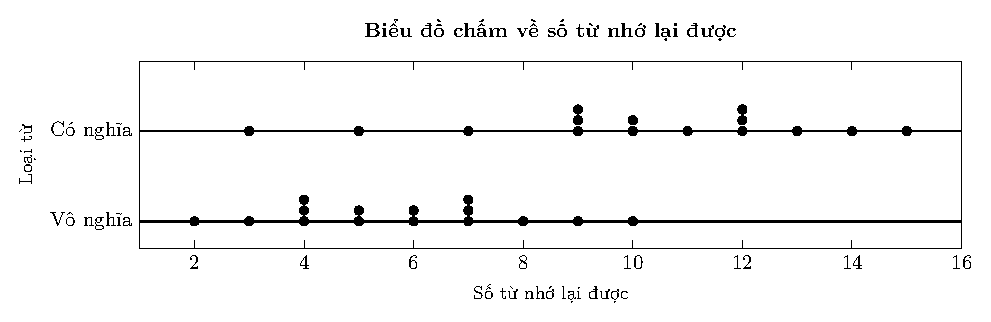
\includegraphics[width=.92\linewidth]{../figures/fhsm_2009_p75_1_vi.pdf}
    \end{center}

    \begin{scriptlist}
      \item [Giáo viên:] Nhìn vào biểu đồ chấm, với loại từ nào thì học sinh nhìn chung có khả năng ghi nhớ tốt hơn? Em biết điều đó bằng cách nào? Hãy đưa ra lí do cụ thể cho câu trả lời của em.
      
      \item [Học sinh A:] Nhiều học sinh được giao từ có nghĩa đạt kết quả tốt hơn. Với nhóm học sinh được giao từ vô nghĩa, số từ nhớ lại cao nhất là $10$. Có bảy học sinh được giao từ có nghĩa nhớ lại hơn $10$ từ, trong khi $10$ là kết quả cao nhất của toàn bộ học sinh được giao từ vô nghĩa. \vspace{\baselineskip}
      
      \item [Học sinh B:] Đúng, nhưng cũng có một số học sinh được giao từ có nghĩa đã không làm tốt. Một bạn chỉ nhớ được ba từ; một bạn khác chỉ nhớ được năm từ; và một bạn nữa chỉ nhớ được bảy từ. Những giá trị này có vẻ thấp đối với nhóm từ có nghĩa.
      
      \item [Học sinh C:] Đúng vậy, và có vài khoảng trống ở phần thấp của phân bố dữ liệu từ có nghĩa, nhưng không nhiều như thế trong phân bố dữ liệu từ vô nghĩa. Nhiều học sinh được giao từ vô nghĩa nhớ lại từ ba đến bảy từ, còn chỉ vài học sinh được giao từ có nghĩa nhớ lại từ ba đến bảy từ.\vspace{2\baselineskip}
      
      \item [Giáo viên:] Em có thể nói cụ thể hơn không?
      
      \item [Học sinh C:] À, ba trong số mười lăm học sinh được giao từ có nghĩa nhớ lại từ ba đến bảy từ. Như vậy chỉ là $20$ phần trăm. Với nhóm học sinh dùng từ vô nghĩa, mười một trong số mười lăm em, tức hơn $73$ phần trăm, nhớ lại được chừng ấy từ. Nếu tính thêm học sinh chỉ nhớ lại hai từ vô nghĩa, thì mười hai trong số mười lăm học sinh này, tức $80$ phần trăm, nhớ lại từ hai đến bảy từ, trong khi chỉ $20$ phần trăm học sinh được giao từ có nghĩa ở mức thấp như vậy. Thật ra, cả mười lăm học sinh dùng từ vô nghĩa đều nhớ lại từ hai đến mười từ, nhưng chỉ tám học sinh được giao từ có nghĩa ở mức thấp như vậy.\vspace{2\baselineskip}
      
      \item [Giáo viên:] Điều đó giống với điều học sinh A đã nói: bảy trong số mười lăm học sinh dùng danh sách từ có nghĩa nhớ lại nhiều từ hơn bất kì học sinh nào dùng danh sách từ vô nghĩa. Điều đó có nghĩa là gần một nửa số học sinh ghi nhớ từ có nghĩa đạt kết quả tốt hơn toàn bộ học sinh được giao từ vô nghĩa.\vspace{\baselineskip}
      
      \item [Giáo viên:] Hãy thử xác định giá trị điển hình cho số từ nhớ lại của mỗi danh sách. Các em đề xuất dùng đại lượng nào?
      
      \item [Học sinh D:] Ta có thể tìm số trung bình nhớ lại cho mỗi danh sách.
      
      \item [Giáo viên:] Vì sao em đề xuất dùng giá trị trung bình, tức đại lượng cũng được gọi là số trung bình cộng?
      
      \item [Học sinh D:] À, có vẻ như ta luôn tìm số trung bình cộng mỗi khi ta muốn biết giá trị điển hình.
      
      \item [Học sinh E:]  Đúng vậy, đôi khi số trung bình cộng là phù hợp. Nhưng đôi khi ta dùng trung vị làm giá trị điển hình.
      
      \item [Giáo viên:] Trong trường hợp này, em dùng cái nào có quan trọng không?
      
      \item [Học sinh E:] À, trong biểu đồ chấm từ có nghĩa, có ba giá trị trông hơi thấp. Em nghĩ ba giá trị này có thể làm số trung bình cộng thấp hơn giá trị điển hình. Vì vậy, em sẽ dùng trung vị thay cho số trung bình cộng.\vspace{\baselineskip}
      
      \item [Giáo viên:] Rất tốt. Khi nhìn thấy đồ thị dữ liệu như biểu đồ chấm của nhóm từ có nghĩa, ta nói hình dạng của phân bố dữ liệu là lệch trái. Như học sinh E đã nói, khi phân bố dữ liệu lệch trái, số trung bình cộng thường nhỏ hơn giá trị mà ta có thể xem là điển hình cho dữ liệu. Vì lí do này, trung vị có thể phản ánh tốt hơn số từ điển hình mà học sinh dùng danh sách từ có nghĩa nhớ lại. Vậy em sẽ đề xuất giá trị nào làm giá trị điển hình cho số từ được nhớ lại bởi học sinh dùng danh sách từ vô nghĩa?\vspace{2\baselineskip}
      
      \item [Học sinh E:] Phân bố dữ liệu của danh sách từ vô nghĩa trông khá đều. Em nghĩ điều này cho thấy nó có hình dạng đối xứng. Vì vậy, có lẽ ta có thể dùng số trung bình cộng hoặc trung vị cho dữ liệu này. Vì ta đang dùng trung vị cho nhóm từ có nghĩa, và sẽ không hợp lí nếu so sánh số trung bình cộng của nhóm này với trung vị của nhóm kia, em cũng sẽ dùng trung vị cho nhóm từ vô nghĩa.\vspace{\baselineskip}
      
      \item [Giáo viên:] Các em nghĩ sao? Điều gì xảy ra khi chúng ta sử dụng trung vị?
      
      \item [Học sinh D:] Máy tính của em cho trung vị của nhóm từ có nghĩa là $10$, còn trung vị của nhóm từ vô nghĩa là $6$.
      
      \item [Giáo viên:] Nếu chúng ta không có giá trị dữ liệu, mà chỉ biết trung vị thì sao? Trung vị cho ta biết điều gì về dữ liệu?
      
      \item [Học sinh D:] Trung vị chia dữ liệu làm đôi.\vspace{\baselineskip}
      
      \item [Giáo viên:] Đúng thế, vậy nếu trung vị là mười từ đối với dữ liệu từ có nghĩa, ta có thể nói gì về phần còn lại của dữ liệu?
      
      \item [Học sinh F:] Khoảng một nửa số học sinh được giao danh sách từ có nghĩa nhớ được ít hơn mười từ, và khoảng một nửa nhớ được nhiều hơn mười từ.\vspace{\baselineskip}
      
      \item [Giáo viên:] Khi so sánh hai trung vị, em sẽ kết luận điều gì?
      
      \item [Học sinh F:] Trung vị của nhóm từ có nghĩa là mười từ, còn trung vị của nhóm từ vô nghĩa là sáu từ. Mười lớn hơn sáu, nên học sinh được giao từ có nghĩa nhìn chung làm tốt hơn học sinh được giao từ vô nghĩa.\vspace{\baselineskip}
      
      \item [Giáo viên:] Đây là một nhận xét thú vị. Một cách nhìn khác về điều này là nói rằng chênh lệch giữa hai trung vị là bốn từ. Vì vậy, học sinh được giao từ có nghĩa thường nhớ lại nhiều hơn học sinh được giao danh sách từ vô nghĩa bốn từ.\vspace{\baselineskip}
      
      \item [Giáo viên:] Nếu với dữ liệu này ta chỉ báo cáo trung vị, thì còn thiếu thông tin gì về số từ được nhớ lại?
        
      \item [Học sinh G:] Nếu chỉ biết trung vị, em không biết số từ thực sự được mỗi học sinh nhớ lại. Lấy dữ liệu của nhóm từ có nghĩa làm ví dụ. Nếu điều duy nhất em biết là trung vị của số từ nhớ lại bằng mười từ, thì em thật sự không biết về những giá trị khác nhau đã thực sự xuất hiện. Chẳng hạn, nhìn vào học sinh chỉ nhớ được ba từ, ba từ khác xa mười từ.\vspace{\baselineskip}
      
      \item [Giáo viên:] Vậy, học sinh G, ý tưởng em đang nói đến được gọi là gì?
      
      \item [Học sinh G:] Số từ được nhớ lại không giống nhau ở từng học sinh. Em nghĩ đây là ý tưởng về biến thiên trong dữ liệu, điều chúng ta đã nói trước đây.
      
      \item [Giáo viên:] Đúng, em nói đúng. Trong thống kê, ta quan tâm đến việc biểu diễn dữ liệu bằng giá trị điển hình, chẳng hạn trung vị, nhưng ta cũng quan tâm đến việc tóm tắt mức độ biến thiên trong dữ liệu. Có ai có đề xuất gì về cách ta có thể làm việc này không?
      
      \item [Học sinh H:] Ta có thể tìm khoảng biến thiên. Em nghĩ đại lượng này cho ta biết điều gì đó về mức độ biến thiên. Khoảng biến thiên của danh sách từ có nghĩa là $12$. Khoảng biến thiên của danh sách từ vô nghĩa là $8$.
      
      \item [Giáo viên:] Vậy, các khoảng biến thiên gợi ra điều gì về biến thiên trong dữ liệu?
      
      \item [Học sinh H:] Chênh lệch lớn nhất giữa hai giá trị bất kì từ danh sách từ có nghĩa là mười hai từ, còn chênh lệch lớn nhất giữa hai giá trị bất kì từ danh sách từ vô nghĩa là tám từ. Điều này cho thấy số từ được nhớ lại ở danh sách từ có nghĩa biến thiên nhiều hơn so với ở danh sách từ vô nghĩa.\vspace{\baselineskip}
      
      \item [Học sinh I:] Đúng vậy, nhưng giá trị nhỏ nhất của nhóm từ có nghĩa có vẻ thật sự thấp. Vì lí do này, em không nghĩ mình sẽ dùng khoảng biến thiên. Thay vào đó, em nghĩ ta nên tìm tứ phân vị và dùng khoảng tứ phân vị (IQR). Khi đó, em đang so sánh mức độ biến thiên ở phần giữa của mỗi nhóm.\vspace{\baselineskip}
      
      \item [Giáo viên:] Em tìm IQR như thế nào?
      
      \item [Học sinh I:] Trước hết, ta phải tìm tứ phân vị thứ nhất và tứ phân vị thứ ba cho mỗi nhóm dữ liệu. Sau đó, ta tìm khoảng biến thiên giữa hai tứ phân vị. Ta lấy tứ phân vị thứ ba trừ tứ phân vị thứ nhất.
      
      \item [Giáo viên:] Được. Cả lớp hãy tìm tứ phân vị và khoảng tứ phân vị.\vspace{\baselineskip}
      
      \item [Học sinh J:] Với nhóm từ có nghĩa, máy tính của em cho tứ phân vị thứ nhất là chín từ và tứ phân vị thứ ba là mười hai từ. Vậy IQR bằng ba từ. Với nhóm từ vô nghĩa, tứ phân vị thứ nhất là bốn từ và tứ phân vị thứ ba là bảy từ. Vậy IQR bằng ba từ. Hai IQR bằng nhau, nên mức độ biến thiên trong $50$ phần trăm giữa của dữ liệu là tương tự nhau ở cả nhóm từ có nghĩa lẫn nhóm từ vô nghĩa.\vspace{\baselineskip}
      
      \item [Học sinh K:] Máy tính của em cho năm đại lượng với mỗi nhóm: giá trị nhỏ nhất, tứ phân vị thứ nhất, trung vị, tứ phân vị thứ ba, và giá trị lớn nhất. Em nghĩ ta có thể có một đồ thị gọi là biểu đồ hộp và râu bằng cách dùng năm số này.
      
      \item [Giáo viên:] Đúng, có thể. Khi đưa thêm phân tích giá trị ngoại lai, nó được gọi là biểu đồ hộp hiệu chỉnh.
    \end{scriptlist}

    Lớp học đã sử dụng kết quả từ máy tính để xây dựng các biểu đồ hộp hiệu chỉnh so sánh sau đây:

    \begin{center}
      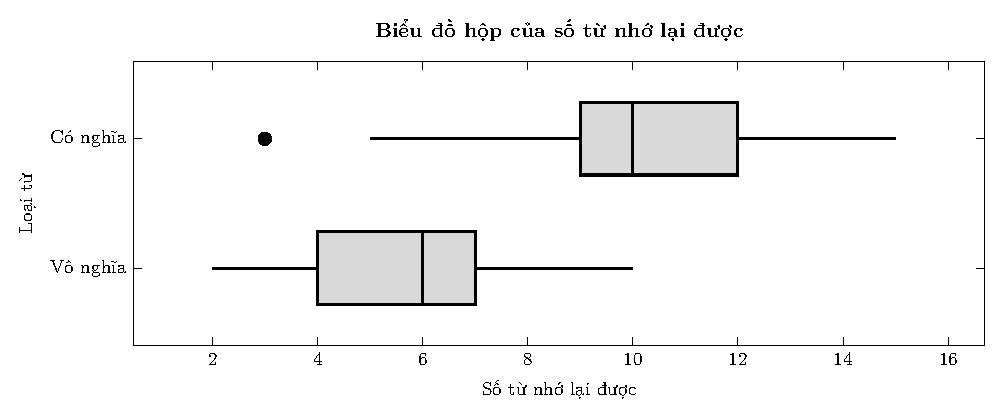
\includegraphics[width=.92\linewidth]{../figures/fhsm_2009_p79_1_vi.pdf}
    \end{center}

    \begin{scriptlist}
      \item [Giáo viên:] Các em có thể dùng kết quả từ biểu đồ hộp để tóm tắt lại thảo luận của chúng ta về câu hỏi này không?
      
      \item [Học sinh M:] Học sinh dùng danh sách từ có nghĩa nhìn chung nhớ lại nhiều từ hơn. Số từ nhớ lại lớn nhất ở nhóm học sinh dùng danh sách từ vô nghĩa là mười. Mười là trung vị của số từ nhớ lại ở nhóm dùng danh sách từ có nghĩa, nên khoảng một nửa học sinh dùng từ có nghĩa nhớ lại nhiều từ hơn bất kì học sinh nào dùng từ vô nghĩa. Với nhóm từ có nghĩa, một học sinh chỉ nhớ lại ba từ, và kết quả này là giá trị ngoại lai, thấp hơn phần nào so với điều có thể kì vọng khi xét phần dữ liệu còn lại. Trung vị của số từ nhớ lại ở nhóm từ có nghĩa là mười, nhiều hơn bốn từ so với trung vị của số từ nhớ lại ở nhóm từ vô nghĩa. Nếu loại giá trị ngoại lai khỏi dữ liệu từ có nghĩa, hai nhóm có vẻ có mức độ biến thiên tương tự nhau. IQR của mỗi nhóm là $3$, cho thấy ở cả từ có nghĩa lẫn từ vô nghĩa, số từ nhớ lại trong $50$ phần trăm giữa của dữ liệu chênh lệch không quá ba từ.\vspace{4\baselineskip}
      
      \item [Giáo viên:] Những kết quả này gợi ý điều gì về trí nhớ và nghĩa?
      
      \item [Học sinh N:] Vì học sinh được giao từ có nghĩa có vẻ đạt kết quả tốt hơn, dữ liệu này gợi rằng từ có nghĩa dễ ghi nhớ hơn.\vspace{\baselineskip}
      
      \item [Giáo viên:] Các em có nghĩ sẽ phù hợp nếu nói rằng mọi học sinh lớp chín đều sẽ cho kết quả đúng hệt như vậy không?
      
      \item [Học sinh O:] Chắc chắn rồi, ghi nhớ từ có nghĩa thì dễ hơn.
      
      \item [Học sinh P:] À, ta sẽ không thu được đúng y hệt các điểm số ấy! Nhưng có thể ta vẫn sẽ thấy rằng từ có nghĩa dễ ghi nhớ hơn.
      
      \item [Giáo viên:] Ta phải cẩn thận với phạm vi suy luận, tức với việc cố khái quát hóa kết quả này cho học sinh lớp chín khác dựa trên dữ liệu này. Phạm vi suy luận phụ thuộc vào việc lớp được nghiên cứu có đại diện cho tất cả lớp chín hay không. Vì ta không biết lớp này được chọn như thế nào, ta không nên cố khái quát hóa kết quả cho tất cả lớp chín hoặc cho mọi học sinh lớp chín. Nếu một nhóm học sinh lớp chín được chọn ngẫu nhiên, khi đó ta có thể thử khái quát hóa kết quả này cho mọi học sinh lớp chín.\vspace{\baselineskip}
      
      \item [Học sinh Q:] Nhưng em tưởng họ đã dùng ngẫu nhiên trong nghiên cứu.
      
      \item [Giáo viên:] Đúng, họ đã dùng. Tuy nhiên, ngẫu nhiên được dùng trong việc phân học sinh vào các nhóm khác nhau. Lí do dùng phân nhóm ngẫu nhiên là để tạo ra hai nhóm có thể so sánh được. Chẳng hạn, ta sẽ không muốn tất cả học sinh giỏi ghi nhớ đều ở cùng nhóm. Bằng cách phân học sinh ngẫu nhiên vào hai nhóm, ta hi vọng cân bằng tác động không chỉ từ khả năng ghi nhớ của học sinh, mà còn từ bất kì biến nào khác có thể liên quan đến số từ được nhớ lại. Dù phân nhóm ngẫu nhiên không bảo đảm các nhóm tương tự nhau, thủ tục này vẫn có khả năng cao tạo ra những nhóm tương tự nhau xét theo mọi biến.
    \end{scriptlist}\vspace{2\baselineskip}

    \textbf{Các yếu tố then chốt của toán học}

    \begin{hanglist}
      \hangitem{Luận với thống kê và xác suất---Phân tích dữ liệu}
    \end{hanglist}

    \textbf{Thói quen luận}

    \begin{hanglist}
      \hangitem{Phân tích bài toán---quyết định liệu cách tiếp cận thống kê có phù hợp hay không; xác định khái niệm, thủ tục hoặc biểu diễn toán học thích đáng; tìm kiếm mẫu hình và quan hệ; đưa ra suy diễn và phỏng đoán sơ bộ}

      \hangitem{Triển khai chiến lược---tổ chức lời giải}\vspace{\baselineskip}

      \hangitem{Tìm kiếm và sử dụng kết nối}

      \hangitem{Phản tư về lời giải---diễn giải lời giải; biện minh hoặc kiểm chứng lời giải; nhận diện phạm vi suy luận}
    \end{hanglist}
  }{}

\ParallelSection
  {Modeling Variability}
  {Mô hình hóa biến thiên}
  {}

\TriPara
  {
    \EN{Probability models reinforce the foundational principle that although an individual observation of a random variable cannot be predicted with certainty, patterns emerge in the frequency of values over a large number of observations. Fostering students' understanding of random variables and probability requires engaging them in the development of both simulation and mathematical probability models. The design of a simulation model requires that students set up a logical sequence of steps for describing the possible outcomes of a random variable. The implementation of a simulation model allows students to both experience and make sense of the notion of the long-run behavior of a random variable and to determine experimental probabilities. The design and implementation of a simulation also provides transitional steps in the development of reasonable mathematical models for describing the long-run behavior of a random variable. Because many probability models involve counting, probability has connections with the Numbers and Measurements strand and the key element of \emph{counting} described in chapter 4. Example 20 considers various developmental strategies for arriving at a solution to a probability problem and illustrates the importance of identifying relevant concepts, procedures, or representations and knowing how a solution can be generalized to a broader class of problems.}
  }
  {
    \VI{Mô hình xác suất củng cố nguyên lí nền tảng rằng tuy từng quan sát riêng lẻ của biến ngẫu nhiên không thể được dự đoán chắc chắn, mẫu hình vẫn xuất hiện trong tần suất xuất hiện của các giá trị qua số lượng lớn quan sát. Việc phát triển sự hiểu biết của học sinh về biến ngẫu nhiên và xác suất đòi hỏi phải cho các em tham gia xây dựng cả mô hình mô phỏng lẫn mô hình xác suất toán học. Thiết kế mô hình mô phỏng đòi hỏi học sinh thiết lập chuỗi bước hợp lí để mô tả các kết quả có thể xảy ra của biến ngẫu nhiên. Việc thực hiện mô hình mô phỏng cho phép học sinh vừa trải nghiệm, vừa hiểu khái niệm hành vi dài hạn của biến ngẫu nhiên và xác định xác suất thực nghiệm. Việc thiết kế và thực hiện mô phỏng cũng cung cấp các bước chuyển tiếp trong quá trình phát triển mô hình toán học hợp lí để mô tả hành vi dài hạn của biến ngẫu nhiên. Vì nhiều mô hình xác suất liên quan đến đếm, xác suất có liên hệ với mạch Số và đo lường cùng yếu tố then chốt \emph{đếm} được trình bày ở Chương 4. Ví dụ 20 xem xét nhiều chiến lược phát triển theo từng mức để đi đến lời giải cho bài toán xác suất, đồng thời minh họa tầm quan trọng của việc nhận diện khái niệm, thủ tục hoặc biểu diễn liên quan và biết cách khái quát hóa lời giải cho lớp bài toán rộng hơn.}
  }{\NOTE{}}

\TriExample
  {
    What Are the Chances? (A)
  }
  {
    \textbf{Task}

    A high school club has fifty members: ten girls and forty boys. The refreshments committee will be formed by selecting two students from the club at random. What is the probability of getting exactly zero girls on the committee? Exactly one girl on the committee? Exactly two girls on the committee? That is, if two students are repeatedly selected at random from the club, how often will exactly no girl be selected? Exactly one girl? Exactly two girls?

    \textbf{In the Classroom (Ninth- to Twelfth-Grade Mathematics Classes)}

    The class is instructed to design a hands-on simulation for estimating the probability for each of the different possible results for the number of girls on the committee. Prior to this activity, students should have had experiences performing simulations by using various random devices and random-number generators in graphing calculators. After the task is read, the teacher can ask the students how they might design a simulation for the situation of choosing two students for the committee and reporting the number of girls on the committee.

    The teacher can lead a discussion to help students design the simulation. Students may propose the use of a standard deck of cards (they would remove two face cards and represent the girls with the ten remaining face cards and the boys with the forty non-face cards). For each trial, they would shuffle the deck several times and then select two cards. The number of face cards selected represents the number of girls on the committee. For the next trial, they would replace the cards in the deck, reshuffle, and select two more cards. Students would need to decide how many trials to perform. From previous experiences, students know that the relative frequencies tend to be close to the actual probabilities if they perform a large number of trials. Together, the class performed a simulation of two hundred trials. The results are summarized in the table at the top of the next page.

    \begin{center}
    \begin{tabular}{|
    >{\centering\arraybackslash}m{1.8cm}|
    >{\centering\arraybackslash}m{1.8cm}|
    >{\centering\arraybackslash}m{3.0cm}|}
    \hline
    Number of Girls & Frequency & Experimental Probability \\
    \hline
    $0$ & $121$ & $.605$ \\
    \hline
    $1$ & $70$  & $.350$ \\
    \hline
    $2$ & $9$   & $.045$ \\
    \hline
        & $200$ & $1.000$ \\
    \hline
    \end{tabular}
    \end{center}

    The experimental probabilities provide estimates for the true probabilities for each of the different possible results and illustrate the long-run relative frequency interpretation of probability.

    \textbf{In the Classroom (High School Statistics Class)}

    Students can revisit this problem in a statistics class after they have learned about tree diagrams and are learning about rules of probability. The class constructed the tree diagram at the right for describing the gender of the two students selected.

    \begin{center}
      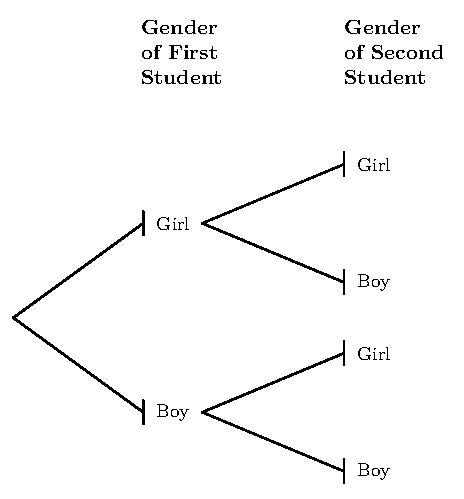
\includegraphics[width=.92\linewidth]{../figures/fhsm_2009_p82_1.pdf}
    \end{center}

    Students are asked to describe the ordered sequence of outcomes for gender that results in the number of girls selected to be 0. For this outcome, the ordered sequence must be---
    \begin{quote}
      Boy selected first and boy selected second.
    \end{quote}

    Students are asked to determine the probability that the first student selected is a boy, which they all agree is
    $$
      \frac{40}{50},
    $$
    or $0.8$.

    They are then asked to think about the probability that the second student selected is a boy, and many said
    $$
      \frac{39}{49}.
    $$\par\vspace*{.25\baselineskip}

    The teacher asks about any assumptions made in determining this probability, and the class agrees that this probability assumes that the first student selected is a boy. The teacher points out that\vspace{\baselineskip}
    $$
      \frac{39}{49}
    $$
    is called a ``conditional'' probability and represents the probability that the second student selected is a boy, given that the first student selected is a boy. The teacher then asks about the probability of the ordered sequence ``Boy selected first and boy selected second.'' A student responds that the sequence can occur only if a boy is selected first and, given that a boy was selected first, a boy is selected second. That is, \vspace{.5\baselineskip}

    \begin{align*}
      P(0\, \text{Girls})
        &= P\left(\text{\parbox{5cm}{Boy selected first and Boy selected second}}\right)\\
        &= P(\text{Boy selected first})\cdot\\
          &\qquad P\left(\text{\parbox{5cm}{Boy selected second given Boy selected first}}\right) \\
        &= \frac{40}{50}\cdot\frac{39}{49}.
    \end{align*}

    The teacher uses this opportunity to present the product rule for probability:
    \begin{align*}
      P&(A\, \text{and}\, B)\\
        &= P(A)P(\text{$B$ given that $A$ has occurred}).
    \end{align*}

    The class expands the tree diagram to show the conditional probabilities for the outcome of gender at each stage of the selection, the ordered sequence of gender, and the number of girls selected for each ordered sequence.

    \begin{center}
      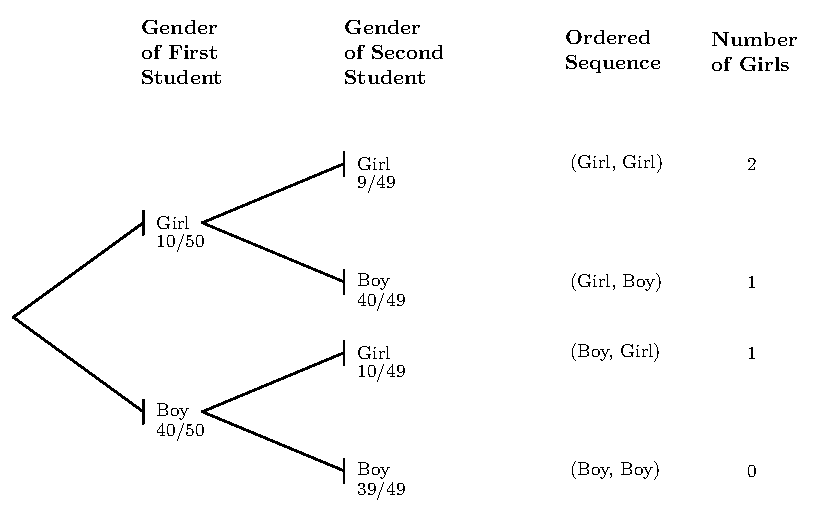
\includegraphics[width=.92\linewidth]{../figures/fhsm_2009_p83_1.pdf}
    \end{center}

    By traversing the tree and using the product rule, the class determines each of the following probabilities:
    \begin{align*}
      P(\text{No Girls})&=(40/50)(39/49)\\
        &\approx .637, \\
      P(\text{One Girl})&=(10/50)(40/49)+(40/50)(10/49)\\
        & \approx .327, \, \text{and} \\
      P(\text{Two Girls})&=P(\text{Girl on First and Girl on Second})\\
        &=(10/50)(9/49)\\
        & \approx .037.
    \end{align*}

    The teacher then asks the class to think about the following question for homework.

    \begin{quote}
      Suppose the gender of the first student selected is not known. We are interested in knowing the probability that the second student selected is a girl (regardless of the gender of the first student selected). This probability is---
      $$ 
      P(\text{Girl selected Second}) =\frac{10}{50}.
      $$

      Can you explain why this is the probability?
    \end{quote}\vspace{.25\baselineskip}

    \textbf{In the Classroom (Twelfth Grade)}

    Students can revisit this problem in the twelfth grade after they have learned counting rules. The class is instructed to use counting rules for determining the probability for each of the different possible results for the number of girls on the committee and to interpret the probabilities. Revisiting the same problem at a higher level gives students an opportunity to make sense of their earlier simulation.

    Students are reminded that
    $$
      C(m,k)=\frac{m!}{k!(m-k)!}
    $$
    counts the number of subsets of size $k$ from $m$ distinct objects.

    For this problem, we get $C(50, 2)$, or $1225$, possible subsets (committees) of size two from the club of fifty students. Since the selection is random, we can assume that each possible committee is equally likely. The number of committees with---
    \begin{quote}
      exactly $0$ girls (and exactly $2$ boys) is $C(10, 0) \cdot C(40, 2)$, or $780$;

      exactly $1$ girl (and exactly $1$ boy) is $C(10, 1) \cdot C(40, 1)$, or $400$;

      exactly $2$ girls (and exactly $0$ boys) is $C(10, 2) \cdot C(40, 0)$, or $45$.
    \end{quote}

    Thus, the mathematical probabilities are as shown in the following table:

    \begin{center}
    \begin{tabular}{|c|c|}
    \hline
    Number of Girls & Probability \\
    \hline
    $0$ & $\frac{780}{1225}\approx .637$ \\
    \hline
    $1$ & $\frac{400}{1225}\approx .327$ \\
    \hline
    $2$ & $\frac{45}{1225}\approx .037$ \\
    \hline
    \end{tabular}
    \end{center}\vspace{.25\baselineskip}

    This example can be used as a rationale for developing the general formula for calculating these types of probabilities when sampling from a finite population. Suppose you have a population with $N$ objects and each object is classified as either a success or a failure. Within the population, $M$ of the objects are successes. You plan to randomly select $n$ objects and to count the number of successes among those selected. For this situation, the number of successes is called a \emph{hypergeometric random variable}, and the probability of obtaining exactly $x$ successes is given by
    $$
      P(x)=\frac{C(M,x)\cdot C(N-M,n-x)}{C(N,n)}.
    $$

    \textbf{\emph{Summary of example 20}}

    Note that the estimated probabilities from the simulation in the first task are close to the probabilities obtained either through counting or using the tree diagram. These latter probabilities indicate that if two members are repeatedly selected at random from the club, then on any one trial, getting exactly zero girls is most likely and would occur approximately $64$ percent of the time. Getting exactly one girl on the committee is fairly common and would occur approximately $33$ percent of the time. In addition, since the probability of getting exactly two girls is less than $.04$, it would be unusual for the committee to have two girls. An examination of this problem from a statistical perspective is described in example 21.

    \textbf{Key Elements of Mathematics}

    \begin{hanglist}
      \hangitem{Reasoning with Statistics and Probability---Modeling variability}

      \hangitem{Number and Measurement---Counting}
    \end{hanglist}

    \textbf{Reasoning Habits}

    \begin{hanglist}
      \hangitem{Analyzing a problem---identifying relevant concepts, procedures, or representations}

      \hangitem{Implementing a strategy---making logical deductions}

      \hangitem{Seeking and using connections}

      \hangitem{Reflecting on one's solution---interpreting a solution; generalizing a solution}
    \end{hanglist}
  }
  {
    Bao nhiêu khả năng? (A)
  }
  {
    \textbf{Nhiệm vụ}

    Câu lạc bộ trung học phổ thông có năm mươi thành viên: mười nữ và bốn mươi nam. Ban phụ trách đồ ăn nhẹ và nước uống sẽ được lập bằng cách chọn ngẫu nhiên hai học sinh từ câu lạc bộ. Xác suất để ban này có đúng không nữ là bao nhiêu? Có đúng một nữ là bao nhiêu? Có đúng hai nữ là bao nhiêu? Nói cách khác, nếu hai học sinh được chọn ngẫu nhiên lặp đi lặp lại từ câu lạc bộ, thì tần suất ban có đúng không nữ là bao nhiêu? Đúng một nữ? Đúng hai nữ?

    \textbf{Trong lớp học (các lớp toán từ lớp 9 đến lớp 12)}

    Lớp được yêu cầu thiết kế mô phỏng thực hành để ước lượng xác suất cho từng kết quả có thể xảy ra về số nữ trong ban. Trước hoạt động này, học sinh nên từng có trải nghiệm thực hiện mô phỏng bằng nhiều thiết bị ngẫu nhiên và bộ sinh số ngẫu nhiên trên máy tính đồ thị. Sau khi nhiệm vụ được đọc lên, giáo viên có thể hỏi học sinh các em sẽ thiết kế mô phỏng như thế nào cho tình huống chọn hai học sinh vào ban và báo cáo số nữ trong ban.\vspace{3\baselineskip}

    Giáo viên có thể dẫn dắt thảo luận để giúp học sinh thiết kế mô phỏng. Học sinh có thể đề xuất dùng bộ bài tiêu chuẩn (các em sẽ bỏ đi hai lá bài hình, rồi dùng mười lá hình còn lại để biểu diễn nữ và bốn mươi lá không hình để biểu diễn nam). Ở mỗi lần thử, các em sẽ xáo bộ bài vài lần rồi rút hai lá. Số lá hình được rút biểu diễn số nữ trong ban. Đến lần thử tiếp theo, các em sẽ đặt lại các lá vào bộ bài, xáo lại, rồi rút thêm hai lá. Học sinh cần quyết định sẽ thực hiện bao nhiêu lần thử. Từ kinh nghiệm trước đó, học sinh biết rằng tần số tương đối thường gần với xác suất thực nếu các em thực hiện số lượng lớn lần thử. Cả lớp cùng thực hiện mô phỏng gồm hai trăm lần thử. Kết quả được tóm tắt trong bảng ở đầu trang tiếp theo.\vspace*{2\baselineskip} 

    \begin{center}
    \begin{tabular}{|
    >{\centering\arraybackslash}m{1.8cm}|
    >{\centering\arraybackslash}m{1.8cm}|
    >{\centering\arraybackslash}m{3.0cm}|}
    \hline
    Số nữ & Tần số & \shortstack{Xác suất\\thực nghiệm} \\
    \hline
    $0$ & $121$ & $.605$ \\
    \hline
    $1$ & $70$  & $.350$ \\
    \hline
    $2$ & $9$   & $.045$ \\
    \hline
        & $200$ & $1.000$ \\
    \hline
    \end{tabular}
    \end{center}

    Xác suất thực nghiệm cung cấp ước lượng cho xác suất thực đối với từng kết quả có thể xảy ra, đồng thời minh họa cách diễn giải xác suất theo tần số tương đối trong dài hạn.\vspace{1\baselineskip}

    \textbf{Trong lớp học (lớp thống kê trung học phổ thông)}

    Học sinh có thể quay lại bài toán này trong lớp thống kê sau khi đã học về sơ đồ cây và đang học về quy tắc xác suất. Cả lớp đã xây dựng sơ đồ cây ở bên dưới để mô tả giới tính của hai học sinh được chọn.

    \begin{center}
      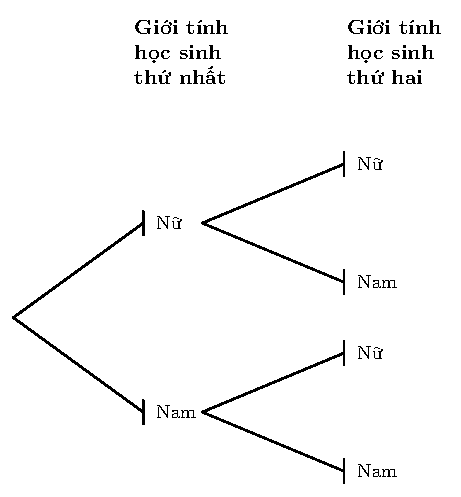
\includegraphics[width=.92\linewidth]{../figures/fhsm_2009_p82_1_vi.pdf}
    \end{center}

    Học sinh được yêu cầu mô tả chuỗi kết quả có thứ tự về giới tính sao cho số nữ được chọn là $0$. Với kết quả này, chuỗi có thứ tự phải là---\vspace{\baselineskip}
    \begin{quote}
      Chọn nam ở lượt thứ nhất và chọn nam ở lượt thứ hai.
    \end{quote}

    Học sinh được yêu cầu xác định xác suất để học sinh thứ nhất được chọn là nam, và tất cả đều đồng ý rằng xác suất đó là
    $$
      \frac{40}{50},
    $$
    hay $0.8$.

    Sau đó, các em được yêu cầu suy nghĩ về xác suất để học sinh được chọn thứ hai là nam, và nhiều em nói rằng xác suất đó là
    $$
      \frac{39}{49}.
    $$

    Giáo viên hỏi các em đã đưa ra giả định nào khi xác định xác suất này, và cả lớp đồng ý rằng xác suất ấy được xác định dựa trên giả định rằng học sinh được chọn ở lượt thứ nhất là nam. Giáo viên chỉ ra rằng
    $$
      \frac{39}{49}
    $$
    được gọi là xác suất ``có điều kiện'' và biểu thị xác suất để học sinh được chọn ở lượt thứ hai là nam, với điều kiện học sinh được chọn ở lượt thứ nhất là nam. Sau đó, giáo viên hỏi về xác suất của chuỗi có thứ tự ``nam được chọn ở lượt thứ nhất và nam được chọn ở lượt thứ hai''. Một học sinh trả lời rằng chuỗi này chỉ có thể xảy ra nếu nam được chọn ở lượt thứ nhất và, với điều kiện nam đã được chọn ở lượt thứ nhất, nam được chọn ở lượt thứ hai. Tức là,
    \begin{align*}
      P(0 \, \text{nữ})
        &= P\left(\text{\parbox{5cm}{Nam được chọn ở lượt 1 và nam được chọn ở lượt 2}}\right)\\
        &= P\left(\text{Nam được chọn ở lượt 1}\right)\cdot\\
          &\qquad P\left(\text{\parbox{5cm}{Nam được chọn ở lượt 2 khi nam đã được chọn ở lượt 1}}\right) \\
        &= \frac{40}{50}\cdot\frac{39}{49}.
    \end{align*}

    Giáo viên nhân cơ hội này giới thiệu quy tắc nhân của xác suất:
    \begin{align*}
      P&(A\, \text{và}\, B)\\
        &= P(A)P(\text{$B$ với điều kiện $A$ đã xảy ra}).
    \end{align*}

    Cả lớp mở rộng sơ đồ cây để thể hiện xác suất có điều kiện cho kết quả về giới tính ở mỗi giai đoạn chọn, chuỗi giới tính có thứ tự, và số nữ được chọn ứng với mỗi chuỗi.

    \begin{center}
      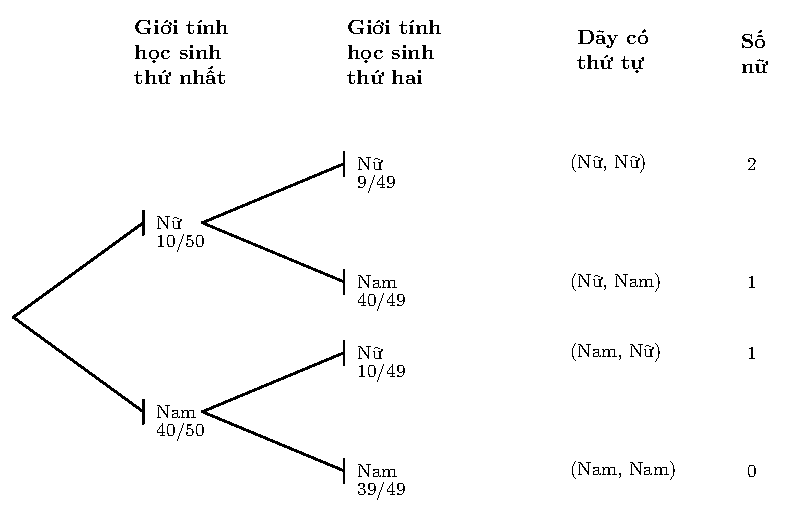
\includegraphics[width=.92\linewidth]{../figures/fhsm_2009_p83_1_vi.pdf}
    \end{center}

    Bằng cách lần theo sơ đồ cây và sử dụng quy tắc nhân, cả lớp xác định từng xác suất sau đây:
    \begin{align*}
      P(\text{Không nữ})
        &=(40/50)(39/49)\\ 
        &\approx .637,\\
      P(\text{Một nữ})
        &=(10/50)(40/49)+(40/50)(10/49)\\
        &\approx .327, \,\text{và} \\
      P(\text{Hai nữ})
        &=P(\text{Nữ ở lượt 1 và nữ ở lượt 2})\\
        &=(10/50)(9/49)\\
        &\approx .037.
    \end{align*}

    Sau đó, giáo viên yêu cầu học sinh suy nghĩ câu hỏi sau như bài tập về nhà.

    \begin{quote}
      Giả sử giới tính của học sinh được chọn ở lượt thứ nhất không được biết. Ta quan tâm đến xác suất để học sinh được chọn ở lượt thứ hai là nữ (không phụ thuộc giới tính của học sinh lượt thứ nhất). Xác suất này là
      $$
      P(\text{Nữ được chọn ở lượt 2})
        =\frac{10}{50}.
      $$

      Em có thể giải thích vì sao đây là xác suất đúng không?
    \end{quote}

    \textbf{Trong lớp học (lớp 12)}

    Học sinh có thể quay lại bài toán này ở lớp 12 sau khi đã học quy tắc đếm. Lớp được hướng dẫn sử dụng quy tắc đếm để xác định xác suất cho từng kết quả có thể xảy ra về số nữ trong ban phụ trách, đồng thời diễn giải xác suất đó. Việc xem lại cùng một bài toán ở mức độ cao hơn tạo cơ hội cho học sinh hiểu mô phỏng mà các em đã thực hiện trước đó.\vspace{1.75\baselineskip}

    Học sinh được nhắc rằng
    $$
      C(m,k)=\frac{m!}{k!(m-k)!}
    $$
    đếm số tập con có kích thước $k$ được chọn từ $m$ phần tử phân biệt.

    Trong bài toán này, ta có $C(50,2)$, tức $1225$, tập con (ban) có kích thước hai được chọn từ câu lạc bộ năm mươi học sinh. Vì việc chọn là ngẫu nhiên, ta có thể giả sử rằng mỗi ban có khả năng được chọn như nhau. Số ban có---\vspace{\baselineskip}
    \begin{quote}
      đúng $0$  nữ (và đúng $2$  nam) là $C(10,0)\cdot C(40,2)$, tức $780$;

      đúng $1$ nữ (và đúng $1$ nam) là $C(10,1)\cdot C(40,1)$, tức $400$;

      đúng $2$ nữ (và đúng $0$ nam) là $C(10,2)\cdot C(40,0)$, tức $45$.
    \end{quote}

    Vì vậy, các xác suất toán học được trình bày trong bảng sau:

    \begin{center}
    \begin{tabular}{|c|c|}
    \hline
    Số nữ & Xác suất \\
    \hline
    $0$ & $\frac{780}{1225}\approx .637$ \\
    \hline
    $1$ & $\frac{400}{1225}\approx .327$ \\
    \hline
    $2$ & $\frac{45}{1225}\approx .037$ \\
    \hline
    \end{tabular}
    \end{center}

    Ví dụ này có thể được dùng như cơ sở để phát triển công thức tổng quát nhằm tính xác suất kiểu này khi lấy mẫu từ tổng thể hữu hạn. Giả sử ta có tổng thể gồm $N$ đối tượng và mỗi đối tượng được phân loại là ``thành công'' hoặc ``thất bại''. Trong tổng thể đó, có $M$ đối tượng là ``thành công''. Ta dự định chọn ngẫu nhiên $n$ đối tượng và đếm số ``thành công'' trong số các đối tượng được chọn. Trong tình huống này, số ``thành công'' được gọi là \emph{biến ngẫu nhiên siêu bội}, và xác suất để thu được đúng $x$ ``thành công'' được cho bởi\vspace{\baselineskip}
    $$
      P(x)=\frac{C(M,x)\cdot C(N-M,n-x)}{C(N,n)}.
    $$

    \textbf{\emph{Tóm tắt Ví dụ 20}}

    Lưu ý rằng xác suất ước lượng từ mô phỏng trong nhiệm vụ đầu tiên gần với xác suất thu được bằng cách đếm hoặc sử dụng sơ đồ cây. Các xác suất sau này cho thấy rằng nếu hai thành viên được chọn ngẫu nhiên lặp đi lặp lại từ câu lạc bộ, thì trong một lần chọn bất kì, việc có đúng không nữ là khả dĩ nhất và sẽ xảy ra xấp xỉ $64$ phần trăm số lần. Việc có đúng một nữ trong ban là khá phổ biến và sẽ xảy ra xấp xỉ $33$ phần trăm số lần. Ngoài ra, vì xác suất có đúng hai nữ nhỏ hơn $0.04$ nên việc ban có hai nữ là trường hợp không thường gặp. Việc xem xét bài toán này từ góc nhìn thống kê được trình bày trong Ví dụ 21.\vspace{3\baselineskip}

    \textbf{Các yếu tố then chốt của toán học}

    \begin{hanglist}
      \hangitem{Luận với thống kê và xác suất---Mô hình hóa biến thiên}

      \hangitem{Luận với số và đo lường---Đếm}
    \end{hanglist}

    \textbf{Thói quen luận}

    \begin{hanglist}
      \hangitem{Phân tích bài toán---xác định khái niệm, thủ tục hoặc biểu diễn toán học thích đáng}

      \hangitem{Triển khai chiến lược---thực hiện suy diễn logic}

      \hangitem{Tìm kiếm và sử dụng kết nối}
      
      \hangitem{Phản tư về lời giải---diễn giải lời giải; khái quát hóa lời giải}
    \end{hanglist}
  }
  {
    Ví dụ 20 được thiết kế theo tiến trình nhiều tầng, nhằm làm nổi bật cách luận xác suất được xây dựng dần từ trực giác đến hình thức. Cùng một bài toán được nhìn qua ba lăng kính: mô phỏng thực nghiệm, mô hình hóa bằng sơ đồ cây với xác suất có điều kiện và quy tắc nhân, rồi quy tắc đếm ở mức độ cao hơn.

    Phần mô phỏng nhấn mạnh cách hiểu xác suất theo tần suất trong dài hạn. Việc yêu cầu học sinh thiết kế phép mô phỏng buộc các em phải mô hình hóa tình huống: quyết định cách mã hóa, chọn thiết bị ngẫu nhiên, quyết định số lần thử, và hiểu vì sao khi số lần thử đủ lớn thì tần suất có xu hướng tiến gần xác suất thực.

    Phần sơ đồ cây đưa học sinh từ trải nghiệm sang cấu trúc. Sự xuất hiện của xác suất có điều kiện ở đây không phải là công thức được cho sẵn, mà là hệ quả tự nhiên của việc rút không hoàn lại. Qua đó, học sinh thấy rõ vì sao quy tắc nhân là cần thiết khi các bước chọn không độc lập với nhau.

    Phần lớp 12 đưa vào quy tắc đếm và mở ra sự khái quát hóa ở trường hợp siêu bội. Đây là bước quan trọng: thay vì chỉ giải bài toán riêng lẻ, học sinh được dẫn đến mẫu hình tổng quát cho việc lấy mẫu từ tổng thể hữu hạn, từ đó đặt nền cho tư duy mô hình và suy luận thống kê.\vspace{\baselineskip}

    \noindent
    \textbf{Ghi chú về có thứ tự và không có thứ tự}\vspace{\baselineskip}

    Trong Ví dụ 20, việc xét thứ tự chọn học sinh không nhằm thay đổi bản chất của bài toán, vì điều bài toán quan tâm rốt cuộc vẫn là số nữ trong ban. Việc đưa thứ tự vào nhằm làm nổi bật cấu trúc của một quá trình ngẫu nhiên nhiều bước. Nhờ đó, xác suất có điều kiện và quy tắc nhân có thể xuất hiện tự nhiên, trước khi học sinh chuyển sang cách tiếp cận không xét thứ tự bằng các quy tắc đếm ở lớp 12.

    \begin{quote}
      Nhưng có phải xét đến thứ tự là làm sai bản chất của bài toán?
    \end{quote}

    \vspace{0.3\baselineskip}
    \noindent
    \emph{Không}. Vì:

    \begin{itemize}
      \item Riêng trường hợp ban có một nữ và một nam, kết quả không xét thứ tự tương ứng với hai chuỗi giới tính có thứ tự: $(\text{nam}, \text{nữ})$ và $(\text{nữ}, \text{nam})$.
      
      \item Khi cộng hai xác suất có thứ tự ấy, ta trở lại đúng xác suất để ban có một nữ:
      $$
      \frac{10}{50}\cdot\frac{40}{49}+\frac{40}{50}\cdot\frac{10}{49}
      = \frac{C(10,1)\cdot C(40,1)}{C(50,2)}.
      $$
    \end{itemize}

    \noindent
    Nói cách khác, việc xét theo thứ tự không làm đổi bài toán; nó chỉ biểu diễn bài toán dưới dạng thuận lợi hơn để làm lộ ra cấu trúc xác suất của quá trình chọn.

    \noindent
    \textbf{Ghi chú về công thức nhân}\vspace{\baselineskip}

    Về mặt trực giác, ta dùng phép nhân trong công thức
    $$
    P(A\cap B)=P(A)P(B\mid A)
    $$
    vì sự kiện ``$A$ và $B$'' ở đây được hiểu như quá trình gồm hai bước liên tiếp: trước hết rơi vào $A$, rồi trong điều kiện $A$ đã xảy ra, tiếp tục rơi vào $B$. Xác suất của toàn bộ quá trình vì thế bằng tỉ lệ đi qua được bước thứ nhất nhân với tỉ lệ đi qua được bước thứ hai. Phép nhân ở đây không phải là quy ước áp đặt từ bên ngoài, mà là hệ quả trực tiếp của cách hiểu cấu trúc của ``và'' trong quá trình xác suất nhiều bước.

    Về mặt toán học, xác suất có điều kiện được lấy làm định nghĩa, và công thức nhân là hệ quả trực tiếp của định nghĩa ấy. Tuy nhiên, trong dạy học, người ta thường dẫn dắt học sinh đến công thức nhân thông qua các quá trình nhiều bước và sơ đồ cây, rồi sau đó mới giới thiệu khái niệm xác suất có điều kiện để hợp thức hóa điều mà trực giác đã nắm được.

    Trong hệ thống Kolmogorov, xác suất có điều kiện không phải là tiên đề mà là định nghĩa. Nó không đặt thêm ràng buộc mới lên xác suất, mà chỉ đặt tên cho biểu thức đã được xác định từ khuôn khổ tiên đề của độ đo xác suất. Vì vậy, công thức xác suất có điều kiện không được gọi là tiên đề, dù nó giữ vai trò nền tảng trong suy luận xác suất.
  }

\ParallelSection
  {Connecting Statistics and Probability}
  {Kết nối thống kê và xác suất}
  {}

\TriPara
  {
    \EN{By incorporating randomness into data collection, probability provides a way to make sense of the variation in sample results from one sample to another. The sampling distribution of a sample statistic (e.g., the sample mean, the sample median, the number of successes or the proportion of successes in the sample) summarizes the long-run behavior of the statistic from repeated random sampling. The sampling distribution provides a mechanism for describing the variation expected in a sample statistic and for determining whether an observed value might be reasonable from chance variation or whether it is more likely due to some other factor. The activity ``Sampling Rectangles'' in \emph{Navigating through Data Analysis in Grades 9--12} (Burrill et al. 2003) illustrates important ideas related to the sampling distribution of the sample mean. The probability distribution developed in example 20 represents the sampling distribution for the number of girls (successes) in a random sample of size two selected from a club of fifty students with ten girls and forty boys. Sampling distributions make crucial links among data analysis, probability, and inferential reasoning in statistics. The following example illustrates foundational ideas underlying the reasoning in inferential statistics by considering the reasonableness of a solution and revisiting initial assumptions.}
  }
  {
    \VI{Bằng cách đưa yếu tố ngẫu nhiên vào việc thu thập dữ liệu, xác suất cung cấp một cách để hiểu sự biến thiên của kết quả mẫu từ mẫu này sang mẫu khác. Phân phối lấy mẫu của thống kê mẫu, chẳng hạn trung bình mẫu, trung vị mẫu, số lần thành công, hay tỉ lệ thành công trong mẫu, tóm tắt hành vi dài hạn của thống kê ấy khi việc lấy mẫu ngẫu nhiên được lặp lại. Phân phối lấy mẫu cung cấp cơ chế để mô tả mức biến thiên được kì vọng ở thống kê mẫu, đồng thời xác định xem giá trị quan sát được có thể được xem là hợp lí do biến thiên ngẫu nhiên hay nhiều khả năng là do yếu tố khác. Hoạt động ``Sampling Rectangles'' trong \emph{Navigating through Data Analysis in Grades 9--12} (Burrill et al. 2003) minh họa ý tưởng quan trọng liên quan đến phân phối lấy mẫu của trung bình mẫu. Phân phối xác suất được xây dựng trong Ví dụ 20 biểu diễn phân phối lấy mẫu của số học sinh nữ, tức số lần thành công, trong mẫu ngẫu nhiên cỡ hai được chọn từ câu lạc bộ gồm năm mươi học sinh, trong đó có mười nữ và bốn mươi nam. Phân phối lấy mẫu tạo ra mối liên hệ then chốt giữa phân tích dữ liệu, xác suất, và suy luận thống kê. Ví dụ tiếp theo minh họa những ý tưởng nền tảng làm cơ sở cho luận trong thống kê suy luận, thông qua việc xem xét tính hợp lí của lời giải và xem xét lại giả định ban đầu.}
  }
  {
    \NOTE{Sự khó hiểu trước hết nằm ở chỗ có quá nhiều tầng đối tượng chồng lên nhau: dữ liệu, mẫu, thống kê mẫu, xác suất, rồi phân phối lấy mẫu. Muốn đọc đoạn văn này cho sáng, cần tách các tầng ấy ra.

    Khi chỉ nhìn vào một mẫu cụ thể, chẳng hạn lấy ngẫu nhiên hai học sinh trong câu lạc bộ rồi đếm số học sinh nữ, kết quả thu được chỉ là một giá trị. Nhưng nếu hình dung việc lấy mẫu ấy được lặp đi lặp lại rất nhiều lần, thì số học sinh nữ trong mẫu sẽ không luôn giống nhau. Có lúc là $0$, có lúc là $1$, có lúc là $2$. Sự thay đổi ấy chính là biến thiên từ mẫu này sang mẫu khác.

    Xác suất được đưa vào để mô tả biến thiên đó. Nó cho phép không chỉ nói rằng các kết quả khác nhau có thể xảy ra, mà còn nói từng kết quả có khả năng xảy ra đến mức nào. Khi đó, thay vì chỉ có kết quả mẫu đơn lẻ, ta có cả bức tranh về tất cả kết quả có thể xuất hiện cùng với khả năng xảy ra của từng kết quả. Bức tranh ấy là phân phối lấy mẫu.

    Vì vậy, phân phối lấy mẫu không phải là phân phối của từng cá nhân trong tổng thể, cũng không phải là phân phối của toàn bộ dữ liệu gốc. Nó là phân phối của đại lượng được tính từ mẫu. Đại lượng ấy có thể là trung bình mẫu, trung vị mẫu, số lần thành công, hay tỉ lệ thành công. Nói ngắn gọn, phân phối lấy mẫu mô tả thống kê mẫu sẽ biến động ra sao nếu việc lấy mẫu ngẫu nhiên được lặp lại nhiều lần.

    Chỗ then chốt nằm ở đây: giá trị quan sát được từ mẫu chỉ thật sự có ý nghĩa khi được đặt vào bối cảnh của phân phối lấy mẫu. Nếu giá trị nằm trong vùng thường gặp của phân phối ấy, thì nó có thể được xem là hợp lí do biến thiên ngẫu nhiên. Nếu nó rơi vào vùng rất hiếm, thì cần nghĩ đến khả năng có nguyên nhân khác tác động, chứ không chỉ do ngẫu nhiên.

    Ví dụ 20 được nhắc tới để làm đúng bước nối đó. Trong ví dụ ấy, xác suất không còn đứng riêng như bài toán đếm thuần túy, mà trở thành công cụ mô tả số học sinh nữ trong mẫu ngẫu nhiên cỡ hai. Nhờ vậy, xác suất bắt đầu gắn trực tiếp với kết quả thống kê có thể quan sát được từ mẫu. Đó chính là chỗ nối giữa phân tích dữ liệu và suy luận thống kê.

    Điểm sâu hơn là: suy luận thống kê không bắt đầu từ việc ``kết luận ngay từ dữ liệu'', mà từ việc hỏi xem dữ liệu quan sát được có bình thường hay bất thường nếu chỉ có ngẫu nhiên tác động. Muốn trả lời câu hỏi đó, phải biết ngẫu nhiên tự nó có thể tạo ra những gì. Phân phối lấy mẫu là công cụ để mô tả điều đó.

    Nếu cần nói cực ngắn, có thể hiểu toàn bộ ý của đoạn văn như sau:

    Lấy mẫu ngẫu nhiên tạo ra biến thiên giữa các mẫu; xác suất mô tả biến thiên ấy; phân phối lấy mẫu cho biết thống kê mẫu thường biến động như thế nào; và nhờ đó mới có cơ sở để đánh giá kết quả quan sát được là hợp lí hay bất thường.}
  }

\TriExample
  {
    What Are the Chances? (B)
  }
  {
    In example 20 we looked at the hypothetical question of selecting two people for a committee and asking what might happen in terms of the number of girls selected. Suppose the president of the club forms the committee and both members are girls. We have now selected a sample and have data on the gender of each student selected. Reporting that the number of girls on the committee is two summarizes the sample data. After hearing the results, the girls in the club questioned the fairness in the selection of the committee. They pointed out that if the committee members were truly chosen at random, then the probability that both are girls is only $.037$ and, because this probability is small, a committee resulting in two girls is unlikely to occur. For this reason, they questioned whether the selection process was fair.

    \textbf{In the Classroom (Twelfth-Grade Mathematics Class)}

    This type of reasoning is the foundation for statistical inference. In this example we assume that the committee-selection process is truly random, and we use this assumption to determine the probability (sampling) distribution for the number of girls on the committee. We then ask how likely the observed result (two girls) is on the basis of this probability distribution. Because this probability is small, the data cast doubt on the assumption that the selection is truly random and thus fair.

    \textbf{Key Elements of Mathematics}

    \begin{hanglist}
      \hangitem{Reasoning with Statistics and Probability---Connecting statistics and probability}
    \end{hanglist}

    \textbf{Reasoning Habits}

    \begin{hanglist}
      \hangitem{Seeking and using connections}

      \hangitem{Reflecting on a solution---considering the reasonableness of a solution; revisiting initial assumptions}
    \end{hanglist}
  }
  {
    Bao nhiêu khả năng? (B)
  }
  {
    Trong Ví dụ 20, ta đã xem xét câu hỏi mang tính giả định: chọn hai người vào ban và hỏi điều gì có thể xảy ra đối với số nữ được chọn. Giả sử chủ tịch câu lạc bộ đã lập ban và cả hai thành viên đều là nữ. Khi đó, ta đã chọn được mẫu và có dữ liệu về giới tính của từng học sinh được chọn. Việc báo cáo rằng số nữ trong ban là hai chính là cách tóm tắt dữ liệu mẫu. Sau khi nghe kết quả, các học sinh nữ trong câu lạc bộ đã đặt câu hỏi về tính công bằng của quá trình lựa chọn ban. Các em chỉ ra rằng nếu thành viên của ban thật sự được chọn ngẫu nhiên, thì xác suất để cả hai thành viên đều là nữ chỉ là $0.037$; và vì xác suất này nhỏ, nên việc ban gồm hai nữ là kết quả ít có khả năng xảy ra. Vì lí do đó, các em nghi ngờ liệu quá trình lựa chọn ban có thật sự công\par\vspace{\baselineskip} bằng hay không.

    \textbf{Trong lớp học (lớp toán lớp 12)}\vspace{\baselineskip}

    Kiểu luận này là nền tảng của suy luận thống kê. Trong ví dụ này, ta giả sử rằng quá trình chọn ban là thật sự ngẫu nhiên, và dùng giả định này để xác định phân phối xác suất (lấy mẫu) cho số nữ trong ban. Sau đó, dựa trên phân phối xác suất này, ta hỏi kết quả quan sát được---tức ban có hai nữ---có khả năng xảy ra đến mức nào. Vì xác suất ấy nhỏ, dữ liệu làm dấy lên nghi ngờ về giả định rằng việc chọn ban là thật sự ngẫu nhiên và do đó là công bằng.

    \textbf{Các yếu tố then chốt của toán học}

    \begin{hanglist}
      \hangitem{Luận với thống kê và xác suất---Kết nối thống kê và xác suất}
    \end{hanglist}

    \textbf{Thói quen luận}

    \begin{hanglist}
      \hangitem{Tìm kiếm và sử dụng kết nối}

      \hangitem{Phản tư về lời giải---xem xét tính hợp lí của lời giải; xem lại giả định ban đầu}
    \end{hanglist}
  }
  {
    Ví dụ 21 chỉ thật sự sáng khi được đặt trong quan hệ trực tiếp với Ví dụ 20. Ở Ví dụ 20, xác suất được dùng để mô tả phân bố của những kết quả có thể xảy ra dưới giả định đã chấp nhận, ở đây là giả định việc chọn ban diễn ra ngẫu nhiên. Ở Ví dụ 21, kết quả cụ thể đã xuất hiện, và câu hỏi chuyển thành: kết quả ấy có còn hợp lí nếu vẫn giữ giả định ban đầu hay không. Chính sự chuyển vai này là điểm cốt lõi. Cùng đại lượng ``số học sinh nữ được chọn'' trước hết được xét như biến ngẫu nhiên có phân phối xác suất, rồi sau đó được đọc như dữ liệu đã quan sát được để đánh giá lại giả định đã đặt ra.

    Điểm quan trọng cần giữ là: xác suất nhỏ không tự động cho phép kết luận rằng quy trình đã không công bằng. Điều mà nó cho phép là kết luận dè dặt hơn và đúng bản chất hơn: nếu kết quả có xác suất rất nhỏ dưới giả định ngẫu nhiên, thì kết quả ấy tạo ra lí do để nghi ngờ giả định ngẫu nhiên ấy. Đây là hình thức sơ khởi của suy luận thống kê. Dữ liệu không chứng minh trực tiếp giả định là sai, nó được dùng để xem giả định ấy đáng tin đến mức nào.

    Vì thế, chỗ nối giữa xác suất và thống kê hiện ra rất rõ. Xác suất cung cấp mô hình cho biến thiên có thể có nếu giả định ban đầu là đúng. Thống kê dùng chính mô hình đó để đánh giá dữ liệu đã quan sát được. Không có bước thứ nhất thì bước thứ hai không có nền để đứng. Cũng vì vậy, Ví dụ 20 và 21 nên được đọc như hai nửa của cùng một ý tưởng, chứ không phải hai ví dụ rời nhau.

    Tình huống kinh điển có thể thay thế đồng thời cả Ví dụ 20 lẫn 21 là thí nghiệm tung đồng xu nhiều lần để kiểm tra giả định đồng xu công bằng. Tình huống này đặc biệt thích hợp cho giảng dạy trên lớp vì có thể thực hiện trực tiếp, dữ liệu được tạo ra ngay trước mắt học sinh, và toàn bộ cấu trúc của cặp Ví dụ 20--21 có thể được tái hiện trong sáng hơn.

    Có thể tổ chức thành hai pha tương ứng.

    Ở pha thứ nhất, đặt giả định rằng đồng xu là công bằng. Khi tung $n$ lần, số lần xuất hiện mặt ngửa là biến ngẫu nhiên. Từ đây có thể lập phân phối xác suất của số lần ngửa. Nếu chọn $n$ nhỏ, chẳng hạn $n=4$ hoặc $n=5$, học sinh có thể tự liệt kê hoặc dùng phép đếm để tìm xác suất của từng kết quả có thể có. Đây là phần tương ứng với Ví dụ 20: câu hỏi trung tâm là nếu giả định ban đầu đúng, thì những kết quả nào có thể xảy ra và với xác suất bao nhiêu. Như vậy, học sinh thấy rõ vai trò của xác suất trong việc mô tả biến thiên của kết quả mẫu.

    Ở pha thứ hai, thật sự tung đồng xu trên lớp, hoặc để một nhóm học sinh tung $20$ lần hay $30$ lần, rồi ghi nhận số lần ngửa thu được. Giả sử kết quả là $18$ lần ngửa trong $20$ lần tung. Lúc ấy câu hỏi thay đổi: nếu đồng xu thực sự công bằng, thì kết quả như vậy có hợp lí không. Muốn trả lời, học sinh phải quay lại phân phối xác suất đã có hoặc dùng nó để tính xác suất của những kết quả ``ít nhất cũng cực đoan như thế''. Đây là phần tương ứng với Ví dụ 21: dữ liệu đã có, và nhiệm vụ là đánh giá dữ liệu ấy dưới giả định ban đầu. Nếu xác suất rất nhỏ, học sinh có cơ sở để nói rằng dữ liệu làm suy yếu giả định đồng xu công bằng.

    Ưu điểm sư phạm của tình huống này là nó làm lộ rất rõ ba tầng:

    \begin{itemize}
      \item giả định ban đầu;
      \item mô hình xác suất dưới giả định ấy;
      \item dữ liệu quan sát được và việc xem lại giả định.
    \end{itemize}

    Nó cũng có lợi thế thực hành mà cặp Ví dụ 20--21 không rõ ràng bằng: học sinh có thể trực tiếp tham gia tạo dữ liệu, nên bước chuyển từ ``khả năng có thể xảy ra'' sang ``điều đã xảy ra'' trở nên sống động hơn nhiều. Chính vì thế, thí nghiệm tung đồng xu là tình huống thay thế rất tốt nếu mục tiêu là dạy mối nối giữa xác suất và suy luận thống kê trong một khuôn khổ gọn, rõ, và có thể triển khai ngay trong lớp.
  }

\ParallelSection
  {Interpreting Designed Statistical Studies}
  {Diễn giải các nghiên cứu thống kê có thiết kế}
  {}

\TriPara
  {
    \EN{Statistical inference involves drawing conclusions from, and making decisions based on, data obtained through designed sample surveys or experiments. Students should understand that the scope of inference for a study is related to the manner in which the data are collected. Data from studies that properly use random selection (sample surveys) or random assignment (experiments) can be used to estimate population characteristics from sample results or to determine whether a result is statistically significant. Sampling distributions offer a way to quantify the uncertainty associated with statistical inference. The reasoning employed in statistical inference is often quite difficult for students; however, using a simulation to create a sampling distribution offers an intuitive way to help students develop inferential reasoning skills. The following example illustrates the reasoning employed in designing and interpreting a simulation for detecting whether a statistically significant difference exists between two groups and presents an interpretation of a solution under uncertain conditions.}
  }
  {
    \VI{Suy luận thống kê liên quan đến việc rút ra kết luận từ dữ liệu và đưa ra quyết định dựa trên dữ liệu thu được qua khảo sát mẫu hoặc thí nghiệm có thiết kế. Học sinh cần hiểu rằng phạm vi suy luận của nghiên cứu gắn với cách dữ liệu được thu thập. Dữ liệu từ nghiên cứu sử dụng đúng chọn ngẫu nhiên (khảo sát mẫu) hoặc phân bổ ngẫu nhiên (thí nghiệm) có thể được dùng để ước lượng đặc trưng tổng thể từ kết quả mẫu, hoặc để xác định liệu kết quả có ý nghĩa thống kê hay không. Phân phối lấy mẫu cung cấp cách định lượng độ bất định gắn với suy luận thống kê. Kiểu luận được dùng trong suy luận thống kê thường khá khó đối với học sinh; tuy nhiên, việc dùng mô phỏng để tạo phân phối lấy mẫu cung cấp con đường trực quan giúp học sinh phát triển kĩ năng suy luận thống kê. Ví dụ tiếp theo minh họa kiểu luận được dùng trong việc thiết kế và diễn giải mô phỏng nhằm phát hiện liệu có tồn tại khác biệt có ý nghĩa thống kê giữa hai nhóm hay không, đồng thời trình bày cách diễn giải lời giải trong điều kiện bất định.}
  }
  {
    \NOTE{Suy luận thống kê được đặt ở đây trên hai loại nghiên cứu được thiết kế: khảo sát mẫu và thí nghiệm. Điểm cần phân biệt là khảo sát mẫu dựa vào chọn mẫu ngẫu nhiên để đi từ mẫu về tổng thể, còn thí nghiệm dựa vào phân bổ ngẫu nhiên để so sánh các nhóm và xem khác biệt quan sát được có thể gắn với tác động đang xét hay không. Vì thế, phạm vi của kết luận không thể tách rời cách dữ liệu được tạo ra.

    Phân phối lấy mẫu là công cụ làm cho bước suy luận ấy trở nên khả dĩ. Nó không mô tả bản thân tổng thể, mà mô tả cách thống kê mẫu sẽ biến động nếu việc lấy mẫu hoặc phân bổ được lặp lại theo cùng cơ chế ngẫu nhiên. Nhờ đó, kết quả quan sát được mới có thể được đặt vào bối cảnh: đó là kết quả vẫn thường xuất hiện do ngẫu nhiên, hay là kết quả đủ hiếm để khiến giả định ban đầu cần được xem xét lại.

    Mô phỏng xuất hiện ở đây không phải như loại nghiên cứu thứ ba, mà như phương tiện để làm lộ phân phối lấy mẫu. Khi việc lặp lại lấy mẫu hay phân bổ không thể thực hiện trực tiếp với số lượng lớn, mô phỏng cho phép tái tạo cơ chế ngẫu nhiên ấy nhiều lần và làm cho mức độ bất định trở nên nhìn thấy được. Theo nghĩa đó, mô phỏng là con đường trực quan để học sinh đi từ dữ liệu quan sát được tới suy luận thống kê.}
  }

\TriExample
  {
    Meaningful Words (B)
  }
  {
    \textbf{Task}

    In example 19, the difference between the medians for the number of words recalled (Meaningful -- Nonsense) was four words, and the fact that this difference is positive lends support to the conjecture that students tend to do better recalling meaningful words than they do recalling nonsense words. Random assignment was used to divide the class into two groups in the hope of producing comparable groups. That is, random assignment is likely to produce two similar groups with regard to all variables at the beginning of the study, and the only difference between the two groups at the end of the study is that one received meaningful words to memorize and the other received nonsense words. Probability provides a way to assess the strength of the evidence found in the difference between the medians. Specifically, because random assignment should produce similar groups, is the observed difference between the medians reasonable from the chance variation that occurs from random assignment, or is this difference likely to be due to the fact that one list contained meaningful words and the other list contained nonsense words? 

    Design and implement a simulation to address this question.

    \textbf{In the Classroom (Twelfth-Grade Class)}

    Students are assumed to have had some exposure to random assignment as a method for controlling for confounding variables and for creating comparable groups in an experimental study. After a class discussion, students reasoned that if the different lists (meaningful and nonsense words) have no effect on memorization, then the observed difference between the medians is due only to the variability expected from the random assignment to groups (i.e., due to the fact that student-to-student differences will be present). Note that a similar type of reasoning was employed in example 21 when students assumed that the selection process was truly random.

    If the different lists have no effect on memorization, then a student's score does not depend on whether he or she memorized meaningful words or nonsense words. Consequently, the number of words recalled by a student would be the same regardless of the group assigned. This situation can be simulated by writing each of the thirty scores on index cards (one score per card), shuffling the cards, and dealing out fifteen cards. The fifteen cards dealt represent scores for the meaningful words; the remaining fifteen cards represent the scores for the nonsense words. The median for each group and the difference between the two medians (meaningful -- nonsense) can be determined. Because the original conjecture for this problem is that people will perform better with meaningful words, we are interested in knowing how often this difference is $+4$ or more. Repeating this simulation $100$ times produced the simulated sampling distribution shown in the dotplot below for the difference between the two medians.

    \begin{center}
      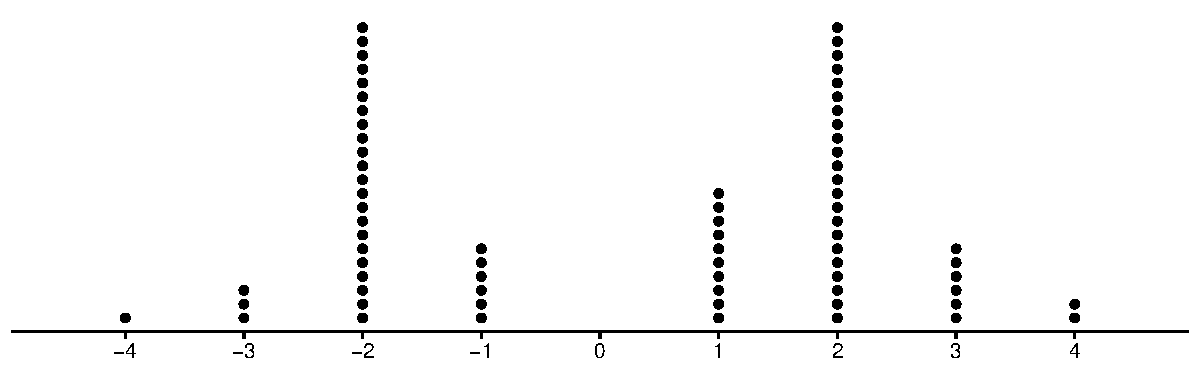
\includegraphics[width=.92\linewidth]{../figures/fhsm_2009_p88_1.pdf}
    \end{center}

    On the basis of this simulation, when no difference is assumed between the effects of the two types of words on memorization, a difference between medians of +4 or more occurred only two times out of $100$ trials. This result suggests that a difference between medians this large ($+4$) or larger is unlikely to occur from chance variation alone. Thus, this difference between medians would be unusual when no difference exists between the effects of the two types of words on memorization; so the use of meaningful words does seem to help when trying to memorize. 

    Because this argument is based on a simulation of only $100$ trials, the statistical reasoning employed here is transitional in nature, from informal to formal. If similar results occurred after performing the simulation with a large number of trials, or if the exact probability distribution for the difference between the medians was available and indicated a similar small probability for a difference of $+4$ or more, then we could say that the difference between the medians is statistically significant (would not be expected as a result of chance variation). In this example the data provide fairly strong evidence that the use of meaningful words does help when trying to memorize.

    (A more detailed illustration of students' reasoning in this problem is presented in the supporting topic book on statistics and probability.)

    \textbf{Key Elements of Mathematics}

    \begin{hanglist}
      \hangitem{Reasoning with Statistics and Probability---Modeling variability; Connecting statistics and probability; Interpreting designed statistical studies}
    \end{hanglist}

    \textbf{Reasoning Habits}

    \begin{hanglist}
      \hangitem{Analyzing a problem---deciding whether a statistical solution is appropriate; making preliminary deductions and conjectures; seeking patterns and relationships}

      \hangitem{Implementing a strategy---making purposeful use of procedures; organizing the solution; making logical deductions}

      \hangitem{Seeking and using connections }

      \hangitem{Reflecting on a solution---revisiting initial assumptions; justifying or validating a solution; interpreting a solution}
    \end{hanglist}
  }
  {
    Từ có nghĩa dễ nhớ hơn? (B)
  }
  {
    \textbf{Nhiệm vụ}

    Trong Ví dụ 19, hiệu giữa hai trung vị của số từ được nhớ lại (từ có nghĩa -- từ vô nghĩa) là bốn từ, và việc hiệu này là số dương đem lại cơ sở ủng hộ cho phỏng đoán rằng học sinh có xu hướng nhớ lại từ có nghĩa tốt hơn từ vô nghĩa. Phân bổ ngẫu nhiên được dùng để chia lớp thành hai nhóm, với hi vọng tạo ra hai nhóm có thể so sánh được. Nói cách khác, phân bổ ngẫu nhiên có khả năng tạo ra hai nhóm tương tự nhau xét theo mọi biến vào lúc bắt đầu nghiên cứu, và khác biệt duy nhất giữa hai nhóm vào lúc kết thúc nghiên cứu là một nhóm nhận danh sách từ có nghĩa để ghi nhớ, còn nhóm kia nhận danh sách từ vô nghĩa. Xác suất cung cấp cách đánh giá độ mạnh của bằng chứng thể hiện qua hiệu giữa hai trung vị. Cụ thể, vì phân bổ ngẫu nhiên được kì vọng tạo ra hai nhóm tương tự nhau, hiệu quan sát được giữa hai trung vị có thể xem là hợp lí do biến thiên ngẫu nhiên nảy sinh từ phân bổ ngẫu nhiên hay không, hay hiệu này nhiều khả năng là do một danh sách gồm từ có nghĩa còn danh sách kia gồm từ vô nghĩa?\vspace{2\baselineskip}

    Hãy thiết kế và thực hiện mô phỏng để xử lí câu hỏi này.

    \textbf{Trong lớp học (lớp 12)}

    Giả định rằng học sinh đã từng tiếp xúc ở mức nhất định với phân bổ ngẫu nhiên như phương pháp kiểm soát biến nhiễu và tạo ra các nhóm có thể so sánh được trong nghiên cứu thực nghiệm. Sau thảo luận trong lớp, học sinh luận rằng nếu các danh sách khác nhau, tức từ có nghĩa và từ vô nghĩa, không có ảnh hưởng đến việc ghi nhớ, thì hiệu quan sát được giữa hai trung vị chỉ do biến thiên được kì vọng từ việc phân bổ ngẫu nhiên vào các nhóm, tức do thực tế là khác biệt giữa học sinh với học sinh vẫn sẽ tồn tại. Lưu ý rằng kiểu luận tương tự đã được sử dụng trong Ví dụ 21, khi học sinh giả định rằng quá trình lựa chọn là thật sự ngẫu nhiên.

    Nếu các danh sách khác nhau không có ảnh hưởng đến việc ghi nhớ, thì điểm số của học sinh không phụ thuộc vào việc em ấy ghi nhớ từ có nghĩa hay từ vô nghĩa. Do đó, số từ học sinh ấy nhớ lại sẽ như nhau bất kể được phân vào nhóm nào. Tình huống này có thể được mô phỏng bằng cách viết từng điểm số trong ba mươi điểm số lên thẻ ghi chú, mỗi thẻ một điểm số, rồi xáo các thẻ và chia ra mười lăm thẻ. Mười lăm thẻ được chia ra biểu diễn điểm số của nhóm từ có nghĩa; mười lăm thẻ còn lại biểu diễn điểm số của nhóm từ vô nghĩa. Có thể xác định trung vị của mỗi nhóm và hiệu giữa hai trung vị, tức từ có nghĩa trừ từ vô nghĩa. Vì phỏng đoán ban đầu của bài toán này là người học sẽ làm tốt hơn với từ có nghĩa, nên điều ta muốn biết là hiệu này xuất hiện ở mức $+4$ hoặc lớn hơn thường xuyên đến mức nào. Lặp lại mô phỏng này $100$ lần tạo ra phân phối lấy mẫu mô phỏng được biểu diễn bằng biểu đồ chấm dưới đây cho hiệu giữa hai trung vị.\vspace{1.75\baselineskip}

    \begin{center}
      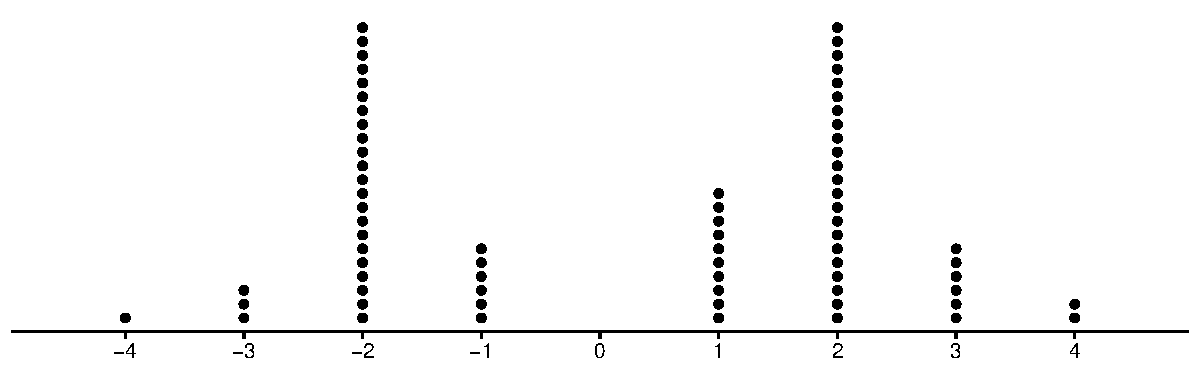
\includegraphics[width=.92\linewidth]{../figures/fhsm_2009_p88_1.pdf}
    \end{center}

    Dựa trên mô phỏng này, khi giả định rằng không có sự khác biệt giữa tác động của hai loại từ đối với việc ghi nhớ, hiệu giữa hai trung vị bằng $+4$ hoặc lớn hơn chỉ xảy ra hai lần trong $100$ lần thử. Kết quả này cho thấy hiệu giữa hai trung vị lớn như vậy ($+4$) hoặc lớn hơn khó có khả năng xảy ra chỉ do biến thiên ngẫu nhiên. Do đó, hiệu giữa hai trung vị như thế là bất thường khi giả định rằng hai loại từ không có tác động khác nhau đến việc ghi nhớ; vì vậy, việc sử dụng từ có nghĩa dường như thật sự giúp ích cho quá trình ghi nhớ.\vspace{\baselineskip}

    Vì lập luận này dựa trên mô phỏng chỉ gồm $100$ lần thử, nên luận thống kê được sử dụng ở đây mang tính chuyển tiếp, từ phi hình thức sang hình thức. Nếu kết quả tương tự xuất hiện khi thực hiện mô phỏng với số lần thử lớn, hoặc nếu có phân phối xác suất chính xác của hiệu giữa hai trung vị và phân phối ấy cũng cho thấy xác suất nhỏ đối với hiệu $+4$ hoặc lớn hơn, thì ta có thể nói rằng hiệu giữa hai trung vị là có ý nghĩa thống kê, tức không được kì vọng xuất hiện do biến thiên ngẫu nhiên. Trong ví dụ này, dữ liệu cung cấp bằng chứng khá mạnh cho thấy việc sử dụng từ có nghĩa giúp cải thiện khả năng ghi nhớ.\vspace{2\baselineskip}

    (Minh họa chi tiết hơn về cách học sinh luận trong vấn đề này được trình bày trong sách chuyên đề bổ trợ về thống kê và xác suất.)\vspace{1\baselineskip}

    \textbf{Các yếu tố then chốt của toán học}

    \begin{hanglist}
      \hangitem{Luận với thống kê và xác suất---Mô hình hóa biến thiên; Kết nối thống kê và xác suất; Diễn giải các nghiên cứu thống kê có thiết kế}
    \end{hanglist}

    \textbf{Thói quen luận}

    \begin{hanglist}
      \hangitem{Phân tích bài toán---quyết định liệu cách tiếp cận thống kê có phù hợp hay không; đưa ra suy diễn và phỏng đoán sơ bộ; tìm kiếm mẫu hình và quan hệ}

      \hangitem{Triển khai chiến lược---vận dụng thủ tục có chủ đích; tổ chức lời giải; thực hiện suy diễn logic}

      \hangitem{Tìm kiếm và sử dụng kết nối}

      \hangitem{Phản tư về lời giải---xem lại giả định ban đầu; biện minh hoặc kiểm chứng lời giải; diễn giải lời giải}
    \end{hanglist}
  }
  {
    Hiệu giữa hai trung vị bằng $+4$ tự nó chưa đủ để kết luận rằng từ có nghĩa giúp ghi nhớ tốt hơn. Điều cần xét không chỉ là độ lớn của hiệu ấy, mà là câu hỏi: nếu không có khác biệt nào giữa hai loại danh sách từ, thì một hiệu như vậy có còn là điều bình thường do cách chia nhóm ngẫu nhiên tạo ra hay không. Chính tại đây suy luận thống kê bắt đầu: kết quả quan sát được chỉ có thể được đánh giá khi đặt trong quan hệ với mô hình của biến thiên ngẫu nhiên. 

    Giả định nền của ví dụ là hai loại danh sách không tạo ra khác biệt thật đối với khả năng ghi nhớ. Khi giữ giả định ấy, điểm số được xem là thuộc về từng học sinh, còn việc một học sinh rơi vào nhóm ``có nghĩa'' hay ``vô nghĩa'' chỉ là hệ quả của phân bổ ngẫu nhiên. Như vậy, câu hỏi trung tâm trở thành: nếu chỉ thay đổi cách chia ngẫu nhiên ba mươi học sinh thành hai nhóm mười lăm và mười lăm, thì hiệu giữa hai trung vị thường dao động ra sao, và giá trị bằng $+4$ hoặc lớn hơn xuất hiện thường xuyên hay hiếm. 

    Mô phỏng được đưa vào để trả lời chính câu hỏi đó. Vì chưa dễ tính trực tiếp xác suất của hiệu giữa hai trung vị ở mức phổ thông, học sinh giữ nguyên ba mươi điểm số đã có, rồi liên tục xáo trộn việc gán chúng vào hai nhóm. Mỗi lần chia lại như vậy tạo ra một “thế giới có thể xảy ra” dưới giả định không có tác động thật, từ đó cho ra một hiệu trung vị mới. Lặp lại nhiều lần sẽ tạo thành phân bố mô phỏng của hiệu giữa hai trung vị. Phân bố ấy đóng vai trò chuẩn tham chiếu: nó cho thấy nếu không có khác biệt thật thì những hiệu nào là bình thường, những hiệu nào là hiếm.

    Biểu đồ chấm vì thế không phải là hình vẽ trang trí thêm vào cho bài toán, mà là cách nhìn thấy trực tiếp biến thiên ngẫu nhiên do phân bổ ngẫu nhiên gây ra. Mỗi chấm là một lần mô phỏng; toàn bộ đám chấm cho biết hiệu trung vị sẽ phân bố ra sao nếu chỉ có ngẫu nhiên tác động. Khi giá trị quan sát được, ở đây là $+4$, rơi vào vùng rất ít xuất hiện của phân bố ấy, nó trở thành kết quả khó giải thích chỉ bằng ngẫu nhiên. Việc chỉ có $2$ lần trên $100$ lần mô phỏng cho hiệu bằng $+4$ hoặc lớn hơn cho thấy kết quả quan sát được là khá hiếm dưới giả định không có tác động. Bởi vậy, dữ liệu tạo ra bằng chứng khá mạnh chống lại giả định ban đầu và nghiêng về phía nhận định rằng từ có nghĩa giúp ghi nhớ tốt hơn.

    Giá trị sư phạm đặc biệt của ví dụ nằm ở chỗ nó làm sáng tỏ toàn bộ xương sống của suy luận thống kê mà không cần đi thẳng vào công thức kiểm định hình thức: bắt đầu từ kết quả quan sát được, đặt giả định nền, mô hình hóa biến thiên ngẫu nhiên dưới giả định ấy, rồi so sánh kết quả quan sát với mô hình để xem nó còn hợp lí hay không. Chính cấu trúc này nối liền dữ liệu thực nghiệm ở Ví dụ 19 với mô hình xác suất và phân phối lấy mẫu ở các ví dụ trước, đồng thời làm cho ``ý nghĩa thống kê'' hiện ra như tính hiếm của kết quả dưới một giả định xác định, chứ không phải như nhãn gắn thêm ở cuối lời giải.
  }

\CloseGrid